\documentclass[12pt]{article}
%%%%%%%%%%%%%%%%%%%%%%%%%%%%%%%%%%%%%%%%%%%%%%%%%%%%%%%%%%%%%%%%%%%%%%%%%%%%%%%%%%%%%%%%%%%%%%%%%%%%%%%%%%%%%%%%%%%%%%%%%%%%%%%%%%%%%%%%%%%%%%%%%%%%%%%%%%%%%%%%%%%%%%%%%%%%%%%%%%%%%%%%%%%%%%%%%%%%%%%%%%%%%%%%%%%%%%%%%%%%%%%%%%%%%%%%%%%%%%%%%%%%%%%%%%%%
\usepackage[utf8]{inputenc}
\usepackage[T1]{fontenc}
\usepackage{textcomp}
\usepackage{graphicx}
\usepackage{color}
%\usepackage{mathpazo} % TEMPORAIRE: fonte Palatino non disponible sans tlmgr
\usepackage{setspace}
\usepackage{etoolbox}
\AtBeginEnvironment{table}{\singlespacing}
\usepackage{amsmath}
\usepackage{booktabs}
%\usepackage{siunitx}          % decimal alignment in tables (inactive until used)
% To activate: install siunitx via tlmgr, then uncomment above and
% replace column type r/c with S[table-format=1.3] in tabular spec,
% e.g. \begin{tabular}{l S[table-format=1.3] S[table-format=1.3]}
% Cells with text (headers, notes) need \multicolumn{1}{c}{...} to override S.
\usepackage{amssymb}

\usepackage{placeins} % peut etre à enlever plus tard

\usepackage{longtable}
\usepackage{threeparttable}
\usepackage[round, authoryear]{natbib}
\usepackage{float}
\usepackage{caption}
\captionsetup{font={small,singlespacing}, labelsep=colon, labelfont=normalfont}
\captionsetup[figure]{justification=justified, singlelinecheck=false}
\captionsetup[table]{justification=justified, singlelinecheck=false}
\usepackage{tabularx}
\usepackage{pdflscape}   % landscape pages for wide tables (\begin{landscape})
\usepackage[pagebackref=true, colorlinks=true, citecolor=black, linkcolor=blue, urlcolor=blue]{hyperref}

%juste pouir que la t able des matoières fasse une page : 
% Compact table of contents

\usepackage{tocloft}

% Table of contents spacing: compact but not too tight
\setlength{\cftbeforesecskip}{4pt}
\setlength{\cftbeforesubsecskip}{2pt}


\renewcommand{\cftsecfont}{\normalsize\bfseries}
\renewcommand{\cftsubsecfont}{\small}
\renewcommand{\cftsecpagefont}{\normalsize\bfseries}
\renewcommand{\cftsubsecpagefont}{\small}


\onehalfspacing
\setlength{\oddsidemargin}{0.01702in}
\newenvironment{proof}[1][Proof]{\noindent\textbf{#1.} }{\ \rule{0.5em}{0.5em}}
\setlength{\textwidth}{16.3cm}
\setlength{\textheight}{21.25cm}
\setlength{\topmargin}{-0.307in}
\DeclareMathOperator*{\Min}{Min}
\interfootnotelinepenalty=10000

\begin{document}

% AI DISCLOSURE + RESPONSIBILITY STATEMENT (2026-05-19)
% À activer pour soumission journal — conserver en commentaire pour le mémoire M2.
%
% \textit{AI disclosure.} This paper used large language model (LLM) assistants
% for the following specific tasks: code formatting and debugging of the R
% estimation script (\texttt{beta17.R}), \LaTeX{} typesetting, stylistic language
% editing of draft sections, and literature search assistance. All economic
% analysis, identification choices, interpretation of results, and conclusions
% are solely my own. I have verified every citation, coefficient, and factual
% claim generated or suggested by AI tools.
%
% \textit{Responsibility statement.} I am the sole author of this paper and
% accept sole responsibility for all content, including any remaining errors.
\author{Presented and Defended by: Robin Masson\thanks{I am grateful to Cem \"{O}ZG\"{U}ZEL for his supervision, sustained feedback, and guidance throughout this research.} \\
{\scriptsize \textsl{Universit\'{e} Paris 1 -- \'{E}cole d'\'{E}conomie de la Sorbonne}}\\
{\scriptsize \textsl{Master 2 Development Economics}}\\
{\scriptsize \textsl{Supervised by: Cem \"{O}ZG\"{U}ZEL}}}

% Ancien titre (conservé pour le mémoire M2, trop long pour soumission journal) :
% One City Burns, Another May Pay? Rental Price Differentials Along Migration Networks after the Williams Lake Wildfire
\title{The Impact of Wildfire Evacuation on Rental Prices: Evidence from Canada}
\date{May 2026}
\maketitle

\begin{abstract}
\begin{singlespace}

When wildfires displace households, nearby cities absorb evacuees, and rents may follow. I study this using the July~2017 Williams Lake evacuation in British Columbia, exploiting a panel of $131$~Canadian cities from 2008 to~2024. The identification uses a Bartik-style shift-share exposure design that weights cities by their pre-fire migration ties to Williams Lake, with log average two-bedroom rent as the outcome. The baseline reduced-form estimate is $0.818$ log-points, implying a $19$-percent rent increase in the most exposed destination. City-specific trends reduce it to $0.594$. The most demanding test, comparing cities within the same province and year, collapses the estimate to $0.164$, indistinguishable from zero, and post-fire migration flows show no amplification toward high-exposure cities. Pre-existing network connections predict rent trajectories, but provincial dynamics confound the wildfire-specific reading. Disaster-relief policy that ignores receiving cities likely underestimates the full housing-cost burden of climate displacement.

\end{singlespace}
\end{abstract}

\begin{singlespace}
\smallskip
\noindent\textit{Keywords}: Wildfires, Climate-induced displacement, Rental prices, Migration networks, Spatial spillovers

\smallskip
\noindent\textit{JEL}: Q54, R23, R31
\end{singlespace}

\newpage

\begin{center}
\bigskip\vspace*{6in}

\textit{L'universit\'{e} de Paris 1 Panth\'{e}on-Sorbonne n'entend donner aucune approbation
ni d\'{e}sapprobation aux opinions \'{e}mises dans ce m\'{e}moire: elles doivent \^{e}tre consid\'{e}r\'{e}es comme propre \`{a} leur auteur.}

\bigskip\vspace*{0.25in}

\textit{The University of Paris 1 Panth\'{e}on-Sorbonne neither approves nor
disapproves of the opinions expressed in this dissertation: they should be
considered as the author's own.}
\end{center}

\newpage
\begingroup
\setstretch{1.12}
\tableofcontents
\endgroup
\newpage

% =============================================================================
\section{Introduction}
\label{sec:intro}

% --- HOOK (2 paragraphs) -----------------------------------------------
In July~2017, a wildfire forced roughly $11{,}000$ Williams Lake residents to evacuate
with less than $24$~hours of warning. Most ended up in Kamloops, Prince George, and Vancouver, drawn by pre-existing
family ties and prior residence. Williams Lake was not unusual. The 2023 Canadian wildfire season burned more than $17$~million hectares,
placing over $230{,}000$ residents under evacuation orders across six provinces
\citep{ciffc2024, publicsafetycanada2024}. Climate projections suggest seasons like 2023
will become routine. Displaced households do not vanish. They move somewhere. Wherever
enough of them concentrate, they compete for apartments, and rents rise.

The policy response to wildfire displacement currently stops at the burn perimeter.
Emergency management tracks evacuees. Disaster relief flows to affected municipalities.
Reconstruction funds target the origin. Receiving cities, where displaced families
actually compete for housing, sit outside this framework entirely. If rental pressure
from wildfire evacuees is large enough to affect housing affordability, the current
policy boundary is drawn too narrowly.

% --- RESEARCH QUESTION + MAIN FINDING (1 paragraph) ----------------------
This paper estimates whether Canadian cities with stronger pre-existing migration ties to
Williams Lake experienced larger rent increases after the July~2017 evacuation. I use a
Bartik-style exposure index that weights each city by its pre-fire share of Williams Lake
out-migrants, interacted with a post-2017 indicator, and estimate the effect on log
average two-bedroom rents across a balanced panel of $131$~Canadian cities from 2008
to~2024. The baseline reduced-form estimate is $\hat{\pi} = 0.818$ log-points
(s.e.\ $0.216$), implying a $19$~percent post-fire rent differential for Kamloops, the
most exposed destination, or roughly \$160~per month on average over 2017--2024 at 2015 rent levels. The most
credible specification adds province-by-year fixed effects and yields $0.164$
(s.e.\ $0.260$), indistinguishable from zero. Pre-existing migration networks predict
rent patterns, but regional confounds prevent a causal reading.

% --- MAIN RESULTS (3 paragraphs) ------------------------------------------
The baseline estimate, taken at face value, is large. \citet{trojanek2022} find
comparable housing market effects from Ukrainian refugee inflows into Poland, a displacement event
roughly $100$~times larger in absolute terms ($1.5$~million refugees versus $11{,}000$
evacuees). If a shock two orders of magnitude smaller produces similar point estimates,
either the per-capita rental impact of wildfire evacuees is extraordinarily high, or the
estimate reflects something other than the fire. The city-specific trends specification
brings the coefficient to $\hat{\pi} = 0.594$ (s.e.\ $0.175$), still statistically
precise at the one-percent level, but the pre-trend evidence points toward the second
interpretation.

Placebo regressions assigned to fictitious treatment years from 2010 to 2016 yield
significant positive coefficients in the baseline. Exposed cities were already growing
faster before the fire. Province-by-year fixed effects compare only cities within the
same province and year. They collapse the estimate to $0.164$ and render it
insignificant. The Rambachan--Roth breakdown value is $\bar{M}^{*}=0.38$.
At that threshold, post-treatment deviations from the pre-trend reach $38$~percent
of the largest pre-treatment violation, and a zero effect enters the confidence set.
The baseline coefficient conflates a Williams Lake network effect with the broader
British Columbia provincial rent trajectory of the late 2010s.

Annual bilateral migration flows reinforce this reading. Flows from Williams Lake to
the $131$~destination cities do not rise after the fire. They fall ($-95.8$,
s.e.\ $8.9$), consistent with a general contraction of out-migration from Williams Lake
rather than a directed surge toward high-exposure destinations. A placebo test using
Quesnel, a nearby forestry town that did not burn, shows no post-2017 shift. Pre-fire migration networks predict post-fire rent
trajectories, but the mechanism turns out not to be the direct displacement shock
the design was built to detect.

% --- LITERATURE & VALUE ADDED (paragraphes révisés) -----------------------

\iffalse % ======= ANCIENS PARAGRAPHES 7-10 (conservés pour référence) =======
The disaster-housing literature concentrates inside damage zones. \citet{boustan2020}
establish, using a century of American county data, that major natural disasters generate
lasting net out-migration from affected areas, the displacement channel this paper
attempts to trace downstream.
\citet{hennighausen2024} find that home prices rose
$13$~percent within $25$~miles of the 2018 Camp Fire in the six weeks following ignition.
\citet{brennan2024} show that severe floods raise rents for the lowest-income renters in
directly flooded neighbourhoods by roughly $5$~percent in the following year. These are
credible designs, but they cannot separate demand pressure from supply destruction,
insurance payouts, and neighbourhood composition shifts. None traces displaced households
to the cities where they land.

A smaller literature examines receiving markets. \citet{harwood2026} studies US natural
disasters and finds heterogeneous rent effects across income groups in receiving
communities, with lower-income neighbourhoods experiencing persistent rent declines
attributed to renovation financing constraints. Across national borders,
\citet{czerniak2024} finds rent inflation in cities receiving Ukrainian refugees across Europe, and \citet{trojanek2022} document short-run housing market effects of the same crisis in Poland. Both papers study international flows governed by asylum policy, not
domestic displacement through voluntary migration networks. No existing paper applies a
shift-share design to climate-induced displacement within a single national housing
market.

Three things distinguish this paper. By measuring rent responses hundreds of kilometres
from the burn perimeter, it isolates a pure demand channel, free from supply destruction
and risk repricing, that within-zone designs cannot reach. It connects domestic migration
network data to the shift-share framework of \citet{goldsmith2020} and \citet{borusyak2022} and documents
how geographic concentration of exposure strains identification when
the origin is a single small city. The binding constraint for this class
of designs is not the shift-share structure itself but the availability of quasi-random
variation in migration shares across many plausibly uncorrelated origins. Williams Lake,
as a single evacuation event, fails this test.

Section~\ref{sec:literature} situates the paper within the disaster-housing and
shift-share literatures. Section~\ref{sec:data} describes the CMHC rental data, the
Statistics Canada bilateral migration flows, and the Williams Lake evacuation.
Section~\ref{sec:strategy} formalises the exposure index and the identifying assumptions
under \citeauthor{goldsmith2020}'s framework. Section~\ref{sec:channel} tests the
displacement mechanism directly using annual origin-destination flows, the test that most
directly challenges the baseline interpretation. Section~\ref{sec:results} reports the
main rent estimates and the event-study profile. Section~\ref{sec:robustness} presents
the full battery of robustness checks: pre-trend placebos, province-year and region-year
absorption, Rotemberg weight diagnostics, COVID truncation, the Sudbury placebo origin,
and pre-period-only trend adjustment. Section~\ref{sec:conclusion} concludes with what
this exercise implies for future attempts to measure displacement-to-rent transmission
from climate events.
\fi % ======= FIN ANCIENS PARAGRAPHES =========================================

The disaster-housing literature establishes that natural disasters generate
lasting out-migration from affected areas. \citet{boustan2020} document,
using a century of American county data, that major disasters cause persistent
population loss at the origin, which provides the empirical foundation for the
displacement flow this paper traces downstream. For wildfires specifically, home
prices rose $13$~percent within $25$~miles of the 2018 Camp Fire in the six
weeks following ignition \citep{hennighausen2024}. Severe floods raise rents for
lowest-income renters in directly affected neighbourhoods by approximately
$5$~percent in the year after the event \citep{brennan2024}. A wider set of
studies reaches consistent conclusions for hurricanes, coastal flooding, and
earthquakes \citep{Vigdor2008, GallagherHartley2017, OrtegaTaspinar2018}.
Every study in this literature operates inside the damage zone, where supply
destruction, insurance payouts, and neighbourhood composition shifts are
inextricably confounded with demand pressure. None follows displaced households
to the cities where they actually compete for apartments.

A smaller literature examines receiving markets. \citet{harwood2026} finds
heterogeneous rent responses across income groups in United States cities
absorbing disaster-displaced households. Lower-income neighbourhoods experience
persistent rent declines attributed to renovation financing constraints, while
higher-income areas recover more quickly. Cross-border evidence comes
from two large displacement events. \citet{trojanek2022} document short-run
housing-market effects of Ukrainian refugee inflows in Poland, and
\citet{czerniak2024} find suggestive rent pressure across European rental markets
hosting the same flows. Neither study applies a shift-share design, and both
concern international population movements governed by asylum policy rather than
voluntary domestic relocation through pre-existing migration networks.

The theoretical prediction for domestic displacement is standard. In a
spatial equilibrium, a positive demand shock raises rents in proportion to
local supply inelasticity \citep{saiz2010}. The empirical benchmark is
\citet{saiz2007}, who estimates that an inflow equal to $1$~percent of city
population raises rents by approximately $1$~percent in American metropolitan
areas. \citet{gonzalez2013} document comparable effects on house prices in Spain.
British Columbia has mountainous terrain, tight zoning, and short-run supply
inelasticity, so the mechanism predicts non-trivial price effects even from
moderate inflows. This channel differs from climate gentrification, in which
long-run risk-perception shifts revalue lower-elevation or climate-resilient
urban land over decades \citep{keenan2018, bernstein2019}. Climate gentrification
predicts broad area-wide revaluations independent of network proximity to a
specific event. The displacement channel studied here predicts rent increases
concentrated in cities with strong pre-fire migration ties to the origin.

Three things distinguish this paper from this literature. First, by estimating
rent responses hundreds of kilometres from the burn perimeter, the design
isolates a pure demand channel free from supply destruction, risk repricing,
and insurance-driven capital flows that confound within-zone estimates. Second,
this is the first application of the shift-share framework of
\citet{goldsmith2020} and \citet{borusyak2022} to domestic climate displacement,
linking pre-determined bilateral migration networks to receiving-city rent
outcomes. Third, this paper documents precisely where a single-origin design
falls short. With exposure concentrated in one small city, the shift-share
shares are not plausibly uncorrelated across destinations, and the strongest
available test compares only cities within the same province, reducing the
estimate from $0.818$ to $0.164$ without resolving which end of that interval
is correct.

% --- ROADMAP ---------------------------------------------------------------
Section~\ref{sec:data} describes the CMHC rental data, the Statistics
Canada bilateral migration flows, and the Williams Lake evacuation context.
Section~\ref{sec:strategy} formalises the exposure index and the
identifying assumptions under \citeauthor{goldsmith2020}'s framework.
Section~\ref{sec:channel} tests the displacement mechanism directly using
annual origin-destination flows, the test that most directly challenges the
baseline interpretation. Section~\ref{sec:results} presents the main rent
estimates and the event-study profile. Section~\ref{sec:robustness} then works through pre-trend placebos,
province-year and region-year fixed effects, Rotemberg weight diagnostics,
COVID truncation, the Sudbury placebo origin, and the Rambachan--Roth
sensitivity bounds.
Section~\ref{sec:conclusion} concludes.

% =============================================================================
% =============================================================================
% NOTE WRITING SAMPLE PRE-DOC (J-PAL / Harvard / Opportunity Insights)
% Pour transformer ce mémoire en writing sample journal-level, 3 actions :
%
% ACTION 1 — Supprimer §2.1 "Natural disasters and local housing-market effects"
%   → C'est un doublon de l'introduction (Boustan, Hennighausen, Brennan y sont
%     déjà cités avec les mêmes limitations). Supprimer entièrement §2.1.
%
% ACTION 2 — Intégrer le contenu conceptuel de §2.2 dans §4 "Empirical Design"
%   → Les paragraphes sur le benchmark Saiz (2007/2010) et la distinction
%     climate gentrification (Keenan 2018, Bernstein 2019) justifient le design,
%     pas la littérature. Les déplacer en ouverture de §4.
%   → Garder uniquement la phrase-pivot "My paper is the first to trace domestic
%     climate-induced displacement..." dans l'introduction.
%
% ACTION 3 — Activer l'AI disclosure dans \thanks{}
%   → Décommenter le bloc AI disclosure + responsibility statement dans \thanks{}
%     (actuellement en commentaire LaTeX au-dessus de \author{}).
%
% POUR LE MÉMOIRE M2 (tel quel) : §2 est CONFORME aux normes Paris 1.
% La section Background séparée est attendue par le jury. Ne pas modifier.
% =============================================================================
\iffalse  % ============ SECTION 2 MISE EN COMMENTAIRE POUR COMPARAISON ============
% Ancien titre commenté : trop long et redondant avec le contenu de la section.
% \section{Background and Conceptual Motivation}
\section{Conceptual Background}
\label{sec:literature}

% Ancien titre commenté : formulation descriptive, trop proche d'une note de plan.
% \subsection{Natural disasters and local housing-market effects}
\subsection{Disasters and Housing Markets}

This paper measures rent responses in cities located hundreds of kilometres
from the burn perimeter, a channel the existing disaster-housing literature
has not examined. That literature establishes that climate disasters
generate significant and persistent out-migration from directly affected
areas. \citet{boustan2020} document, using a century of American
county-level data, that major natural disasters generate lasting net
out-migration from affected counties, providing the empirical foundation
for the displacement channel I exploit. For wildfires specifically, home transaction prices rose $13$~percent
within $25$~miles of the 2018 Camp Fire in California in the six weeks
after ignition, with effects decaying sharply with distance
\citep{hennighausen2024}. Severe floods raise rents for the
lowest-income renters in directly affected areas by approximately
$5$~percent in the year following the disaster \citep{brennan2024}.
A broader literature documents the housing-market consequences of major
events in directly affected areas \citep{Vigdor2008, GallagherHartley2017,
OrtegaTaspinar2018}. These designs cannot separate demand shocks from
supply destruction, insurance discontinuities, and neighbourhood
composition changes. They do not speak to rental markets in cities
that received displaced households.

% Ancien titre commenté : trop long ; le nouveau titre garde l'idée centrale.
% \subsection{Migration shocks and receiving-city rental markets}
\subsection{Receiving Markets}

This paper is the first to trace domestic climate-induced displacement
through national migration networks to rental markets in distant cities.
The existing literature on receiving markets is limited in scope.
Low-income neighbourhoods in disaster-receiving areas experience rent
declines persisting for several years, while higher-income neighbourhoods
rebound more quickly, a gap attributed to differential access to
renovation financing \citep{harwood2026}. An emerging strand examines cross-border
displacement: \citet{trojanek2022} document significant short-run effects of Ukrainian refugee inflows on the Polish housing market, and \citet{czerniak2024} find suggestive but imprecisely estimated rent pressure across European rental markets. These contributions study either short-distance spillovers from
a single coastal event or international geopolitical flows. None uses
predetermined domestic migration networks to estimate receiving-city
rent effects at the national scale.

Two features of wildfire displacement distinguish my setting from the
international immigration literature. First, the evacuation shock is
sudden and unanticipated, leaving no time for supply-side adjustment.
Second, displaced households are pushed out by an exogenous event rather
than drawn by destination-city attractiveness, removing the standard
selection concern that migrants sort into high-rent markets. The
relevant network link encompasses both Williams Lake residents with social ties
in receiving cities and former residents of those cities who had previously
moved to Williams Lake and who return upon evacuation; these two groups may
differ in their elasticity of return and in the rental demand they generate. The
theoretical prediction is standard: in a spatial equilibrium framework,
a positive housing-demand shock raises rents in cities where supply is
inelastic \citep{saiz2010}. The empirical benchmark is \citet{saiz2007},
who finds that an inflow equivalent to $1$~percent of city population
raises rents by approximately $1$~percent across American metropolitan
areas; \citet{gonzalez2013} document comparable effects on house prices in Spain.
The supply-elasticity estimates in \citet{saiz2010} imply that the rent response is two to three times
larger in physically constrained cities. For the British Columbia rental
market, characterised by mountainous terrain, zoning constraints, and
short-run supply inelasticity, this mechanism predicts non-trivial price
effects even from moderate inflows.

A related but distinct mechanism is \emph{climate gentrification}: the
revaluation of lower-elevation or otherwise climate-resilient urban land
driven by long-run risk-perception shifts \citep{keenan2018, bernstein2019}.
Although both mechanisms link climate events to housing-cost changes, they
operate through different channels and at different timescales: climate
gentrification unfolds over decades as households update beliefs about
chronic flood or heat exposure, while the displacement shock studied here
operates over months through sudden demand pressure along pre-existing
migration networks. The two channels are empirically distinguishable
because the latter predicts rent increases concentrated in cities with
strong pre-fire migration links to Williams Lake, whereas the former
predicts broad revaluations of lower-risk areas independent of network
proximity to the event.

\fi  % ============ FIN SECTION 2 COMMENTÉE =====================================

% =============================================================================
% DÉCISIONS DE NETTOYAGE DES DONNÉES — résumé des 7 choix matériels (2026-05-19)
% Toutes documentées dans le texte des §3.2 et §3.5 ; récapitulatif ici
% pour la soutenance et la vérification par les referees.
%
% 1. 8 sous-géographies biprovinciales supprimées (éviter le double comptage)
% 2. Marchés CMHC sans contrepartie dans la table de migration exclus
% 3. Résidus ruraux provinciaux exclus (pas de correspondance géographique)
% 4. Intersection des deux sources : 145 villes retenues sur 173 initiales
% 5. 13 villes nécessitent une harmonisation de nom non triviale avant merge
% 6. 4 villes biprovinciales traitées avec ajustements spécifiques par province
% 7. 14 villes supprimées pour équilibrer le panel (Belleville, Courtenay,
%    Leamington principal cas de gaps tardifs)
% =============================================================================
% =============================================================================
% Ancien titre commenté : légèrement lourd pour la table des matières.
% \section{Data and Institutional Context}
\section{Data and Context}
\label{sec:data}

% Ancien titre commenté : article défini inutile ; version plus sobre.
% \subsection{The 2017 Williams Lake evacuation}
\subsection{Williams Lake Evacuation}
\label{sec:wl_context}

On July~7, 2017, authorities in Williams Lake, British Columbia issued a
mandatory evacuation order with fewer than $24$~hours' notice, as a
converging firestorm threatened the city during an exceptionally severe
wildfire season. Roughly $11{,}000$ residents were ordered to leave. The
timing was driven by meteorological and fire-propagation conditions, not by
rental-market developments in potential receiving cities, which rules out
anticipatory price adjustment by landlords in destination markets. Because
the order came without warning, displaced households had no time to search
systematically for preferred destinations. They moved toward cities where
they already had family ties, prior employment, or a history of residence.
The empirical design exploits this by measuring pre-fire migration links
between Williams Lake and each Canadian city in the panel.

% Ancien titre commenté : formulation trop procédurale.
% \subsection{Data sources and sample construction}
\subsection{Sources and Sample}
\label{sec:sources_sample}

The panel draws on three Canadian administrative sources. Migration flows
come from Statistics Canada Table~17-10-0141-01 \citep{statcan_migration},
which records annual intercity flows across Census Metropolitan Areas,
Census Agglomerations, and related geographies. These bilateral flows
construct the pre-fire Williams Lake destination shares and allow a
direct test of whether post-fire arrivals from Williams Lake amplified
toward high-exposure destinations. Rental data come from CMHC
Table~34-10-0133-01 \citep{cmhc_rental}, which reports average monthly
rents by market, unit type, and structure type.\footnote{All three data sources are publicly available at no cost under the Statistics Canada Open Licence. The complete replication package, including all code and auxiliary files needed to reproduce every table and figure, is available at \url{https://github.com/Robin-Economist/The-Impact-of-Wildfires-on-Rental-Prices-Evidence-from-Canada}.}
The CMHC Rental Market Survey for 2017 provides the two-bedroom vacancy
rates and rental-universe counts used in the economic calibration in
Section~\ref{sec:economic_calibration}. Centroid coordinates for the
spatial exposure map are computed from the 2021 Census geography boundary
files (Statistics Canada catalogue~92-160-X), accessed via the R package
\texttt{cancensus} \citep{vonBergmann2021}. Bay Roberts, Leamington, and
Cold Lake are geocoded manually from Statistics Canada's 2021 Census
community profiles, while the biprovincial agglomerations of Campbellton
and Hawkesbury are reconstructed from their provincial geography components
to match the migration-table units.

Building the estimation sample requires reconciling two geographic systems
that do not map one-to-one. Starting from the 173 areas in the migration
table, I drop eight biprovincial subgeographies to avoid double-counting.
On the rent side, CMHC markets that correspond to census subdivisions
outside any Census Metropolitan Area or Census Agglomeration have no
counterpart in the migration table and are excluded. Provincial rural
residuals are likewise dropped. The two sources intersect on 145 cities.
Thirteen require non-trivial name harmonisation before merging, and four
biprovincial cities require province-specific adjustments.

The panel runs from 2008 to 2024. Within the 145-city intersecting sample,
the share of city-year observations with non-missing rent averages 98.0\%
from 2008 onward and never falls below 96.5\% in any single year. Coverage
falls sharply before 2008, so extending the window back further would trade
a longer pre-period for a smaller and less stable city sample.

% Ancien titre commenté : trop mécanique ; le nouveau titre indique directement l'objet.
% \subsection{Dependent variable}
\subsection{Rent Measure}

The dependent variable is the logarithm of average monthly rent for
two-bedroom apartments in structures containing three or more units (CMHC
Table~34-10-0133-01). Following \citet{saiz2007}, who uses a two-bedroom
rental measure as the benchmark for primary rental-market conditions in
American metropolitan areas, this segment offers the best compromise
between economic relevance and coverage in the Canadian data. Two-bedroom
rents are non-missing for 98.0\% of city-year observations from 2008
onward, while bachelor and three-bedroom series show materially more
attrition, particularly in smaller cities. Two-bedroom units also provide
a more stable composition proxy than the smallest unit categories, whose
mix shifts as developers respond to land costs. Alternative unit and
structure definitions appear in Appendix Figure~\ref{fig:heterogeneity_coefplot}.

One interpretive caveat applies throughout. Because CMHC average rent
pools long-term controlled leases with new-tenancy rents, and because
British Columbia rent regulations cap annual increases for continuing
tenants, estimates from this series likely understate the market-clearing
response to a demand shock. Wildfire-driven demand shocks manifest first
in new leases, which the CMHC average only partially reflects.

% Ancien titre commenté : trop long et trop technique pour un sous-titre.
% \subsection{Explanatory variable: pre-fire migration shares}
\subsection{Migration Exposure}

The explanatory variable is the pre-fire bilateral migration share
$s_{WL,d}$, defined as the fraction of Williams Lake out-migrants who settled
in destination city~$d$ during the 2016/2017 migration wave:

\begin{equation}
s_{WL,d} =
\frac{
\text{Migrants from Williams Lake to city } d \text{ in 2016/2017}
}{
\text{Total out-migrants from Williams Lake in 2016/2017}
}.
\label{eq:shares}
\end{equation}

Statistics Canada's migration wave runs from July~2016 to June~2017,
placing it entirely before the July~2017 wildfire. Rural residual
destinations are excluded and shares are renormalised to sum to one across
the retained city destinations. Using the wave immediately preceding the
evacuation rather than a multi-year average maximises contemporaneity with
the shock. The concentration of Williams Lake out-migrants in a stable set
of British Columbia cities suggests that alternative window definitions
would yield similar exposure profiles.

Of the 131 cities in the main panel, 43 have a strictly positive pre-fire
share and 88 have zero observed share. A caveat: Statistics Canada suppresses
bilateral cells below its confidentiality threshold, so genuine small flows
toward minor destinations may be recorded as zero. If suppressed cells
concentrate among smaller non-British Columbia cities, the zero-exposure
control group is contaminated by cities with genuine but unobserved positive
exposure, attenuating the estimated differential. The distribution of
positive shares is highly concentrated. Kamloops accounts for 21.2\%,
followed by Vancouver at 17.4\%, Prince George at 9.97\%, Kelowna at
6.91\%, and Quesnel at 6.75\%. Across all 131 cities, the mean share is
0.007 and the median is zero.

Two panel consistency adjustments are straightforward. Williams Lake itself
enters with $s_{WL,d}=0$, since out-migrants from a city are not counted as
returning to it. The two biprovincial agglomerations (Campbellton, Hawkesbury)
report separate CMHC rent series by provincial part but a single merged
migration record; their rent observations are averaged across parts and their
migration share is set to zero, consistent with the dropping of biprovincial
sub-geographies on the migration side.

% Ancien titre commenté : formulation trop spécifique pour la table des matières.
% \subsection{British Columbia housing-policy context}
\subsection{Policy Context}
\label{sec:bc_policy}

Three British Columbia housing-policy changes overlap with the post-2017 estimation
window and may confound the exposure estimates, particularly for Vancouver and other
highly exposed cities. The Foreign Buyers Tax (August~2016) imposed a
15~percent surcharge on residential purchases by foreign nationals in Metro Vancouver,
reducing ownership demand and diverting it partly toward the rental market.
The Speculation and Vacancy Tax (announced 2018, operative from 2019) extended
a similar logic province-wide, adding rental pressure in secondary markets.
The Residential Tenancy Act cap on annual rent increases, applied throughout
the period but tightened in~2023 to a maximum of~2~percent, limits the observable
rent response in tenancies with continuing tenants while leaving new-tenancy rents
unrestricted. These policy changes affect the CMHC average-rent series differentially
across cities: markets with rapid turnover (Vancouver, Kelowna) display faster
adjustment than stable markets with low vacancy. Because the most exposed cities are
disproportionately located in British Columbia and subject to these policies
simultaneously with the wildfire exposure, the identification threat they pose
cannot be eliminated by the baseline design. The Vancouver robustness check in
Section~\ref{sec:vancouver_checks} directly addresses the Vancouver-specific
policy channel. The province-by-year fixed effects in
Section~\ref{sec:prov_year_fe} address the broader provincial policy component.

% Ancien titre commenté : titre trop administratif.
% \subsection{Final sample and descriptive statistics}
\subsection{Sample and Descriptives}

The main estimation sample retains 131 cities over 2008--2024. Of the
145-city intersecting sample, 14 cities have at least one missing observation
in the baseline rent series and are dropped to preserve a balanced panel.
The most exposed among them, Belleville and Courtenay, each account for
0.64\% of Williams Lake's pre-fire out-migrants, so their exclusion is
unlikely to affect any of the estimates. This is confirmed in the
unbalanced-panel exercise in Appendix Table~\ref{tab:robustness_instrument}.
Leamington is the only city with late-period gaps (its rent series drops
out in 2023 and 2024) and remains in the sample since these gaps fall well
after the core treatment window. The panel is nearly balanced: of
$131 \times 17 = 2{,}227$ city-year slots, $2{,}225$ carry non-missing rent
observations.

Average monthly rent is $\$908$, with a median of $\$857$
(Table~\ref{tab:desc_stats}). The within-city standard deviation is
$\$190$, against a between-city standard deviation of $\$229$, indicating
substantial time variation within markets. Exposed cities ($s_{WL,d}>0$,
$N=43$) have higher baseline rents than non-exposed cities ($N=88$) and
faster post-2017 growth: mean rents rose from $\$895$ to $\$1{,}219$ (36\%)
among exposed cities, against 31\% for non-exposed cities. These level
differences motivate city fixed effects in all specifications. The
differential post-2017 pattern is evaluated formally in
Sections~\ref{sec:strategy} and \ref{sec:results}.

% =============================================================================
% TABLE 1 -- DESCRIPTIVE STATISTICS
% =============================================================================
\begin{table}[t]
  \caption{Descriptive Statistics}
  \label{tab:desc_stats}
  \centering\small
  \begin{threeparttable}

    \begin{tabular*}{\linewidth}{@{\extracolsep{\fill}}lrrrrrr}
      \multicolumn{7}{l}{\textit{Panel~A: Summary statistics}} \\[2pt]
      \toprule
      & Obs. & Mean & Median & Std.\ Dev. & Min & Max \\
      \midrule
      Monthly rent (\$)             & 2{,}225 & 908  & 857  & 297   & 384  & 2{,}360 \\
      Log monthly rent              & 2{,}225 & 6.76 & 6.75 & 0.309 & 5.95 & 7.77    \\
      $s_{WL,d}$ (\%, $\times 100$) & 2{,}225 & 0.70 & 0.00 & 2.70  & 0.00 & 21.2    \\
      \bottomrule
    \end{tabular*}

    \bigskip

    \begin{tabular*}{\linewidth}{@{\extracolsep{\fill}}lrrrr}
      \multicolumn{5}{l}{\textit{Panel~B: Average monthly rent (\$) by exposure status and period}} \\[2pt]
      \toprule
      & \multicolumn{2}{c}{Non-exposed} & \multicolumn{2}{c}{Exposed} \\
      \cmidrule(lr){2-3}\cmidrule(lr){4-5}
      & Pre-2017 & Post-2017 & Pre-2017 & Post-2017 \\
      \midrule
      Mean rent (\$)    & 733 & 961 & 895 & 1{,}219 \\
      Std.\ dev.        & 197 & 284 & 240 & 281     \\
      $\Delta$ (\$)     & \multicolumn{2}{c}{228 (31\%)} & \multicolumn{2}{c}{324 (36\%)} \\
      Cities            & \multicolumn{2}{c}{88}  & \multicolumn{2}{c}{43} \\
      Observations      & 792 & 704 & 387 & 342     \\
      \bottomrule
    \end{tabular*}

    \begin{tablenotes}[flushleft]\footnotesize
      \item \textit{Notes:} Unit of observation: city-year.
        Sample: 131 Canadian cities, 2008--2024 (2{,}225 observations).
        Monthly rent is the CMHC average rent for two-bedroom apartments in
        buildings with three or more units (Table~34-10-0133-01).
        $s_{WL,d}$ is the pre-fire share of Williams Lake out-migrants settling
        in city~$d$, from Statistics Canada bilateral flows, wave 2016/2017
        (Table~17-10-0141-01); reported in percentage points ($\times 100$).
        Pre-2017: 2008--2016; post-2017: 2017--2024.
        Exposed cities: $s_{WL,d}>0$ ($N=43$);
        non-exposed: $s_{WL,d}=0$ ($N=88$). Panel B reports raw means by exposure status and period.
    \end{tablenotes}
  \end{threeparttable}
\end{table} 

% Ancien titre commenté : simple correction de style et capitalisation.
% \subsection{Descriptive evidence}
\subsection{Descriptive Evidence}
\label{sec:descriptive}

Exposure is geographically concentrated in British Columbia: most Canadian cities
have no observed pre-fire link to Williams Lake, while the highest shares cluster
in British Columbia (Figure~\ref{fig:spatial_exposure}). Exposed cities show higher
average rents before 2017 and larger post-2017 rent growth than non-exposed cities
(Figure~\ref{fig:rent_evolution}). Appendix
Figures~\ref{fig:rent_distribution} and \ref{fig:treatment_intensity} report
the full rent distribution and the histogram of positive migration shares.

% =============================================================================
% FIGURE -- SPATIAL DISTRIBUTION OF EXPOSURE
% =============================================================================
\begin{figure}[htbp]
  \centering\singlespacing
  \caption{Spatial Distribution of Pre-Fire Migration Exposure}
  \label{fig:spatial_exposure}
  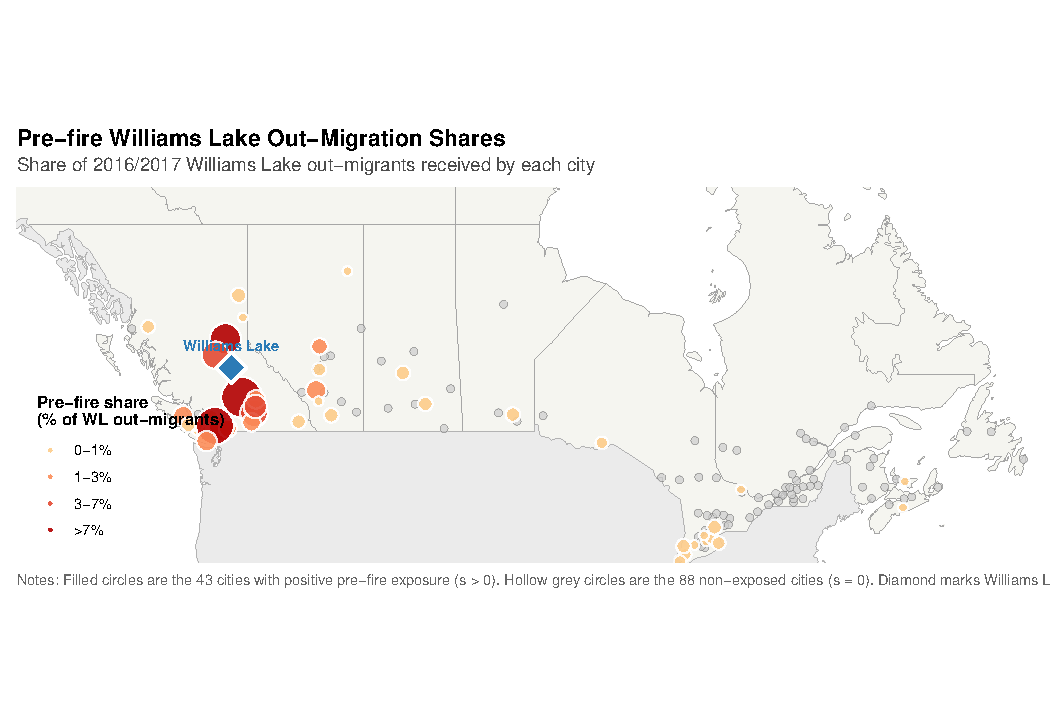
\includegraphics[width=0.92\textwidth]{figures/fig_spatial_exposure_qgis}
  \par\smallskip\begin{minipage}{0.92\textwidth}\setstretch{1.0}\footnotesize\textit{Notes:} Each point is a city in the main estimation sample ($N=131$). Filled
    circles denote the 43 exposed cities ($s_{WL,d}>0$); colour and size are
    proportional to the pre-fire migration share $s_{WL,d}$ (share of 2016/2017
    Williams Lake out-migrants received by each city). Hollow grey circles are the
    88 non-exposed cities ($s_{WL,d}=0$). The diamond marks Williams Lake, British
    Columbia (origin). Pre-fire migration shares are from the Statistics Canada
    2016/2017 internal migration wave.\end{minipage}
\end{figure}

% =============================================================================
% FIGURE -- RENT EVOLUTION OVER TIME
% =============================================================================
\begin{figure}[H]
  \centering\singlespacing
  \caption{Mean Monthly Rent by Exposure Status, 2008--2024}
  \label{fig:rent_evolution}
  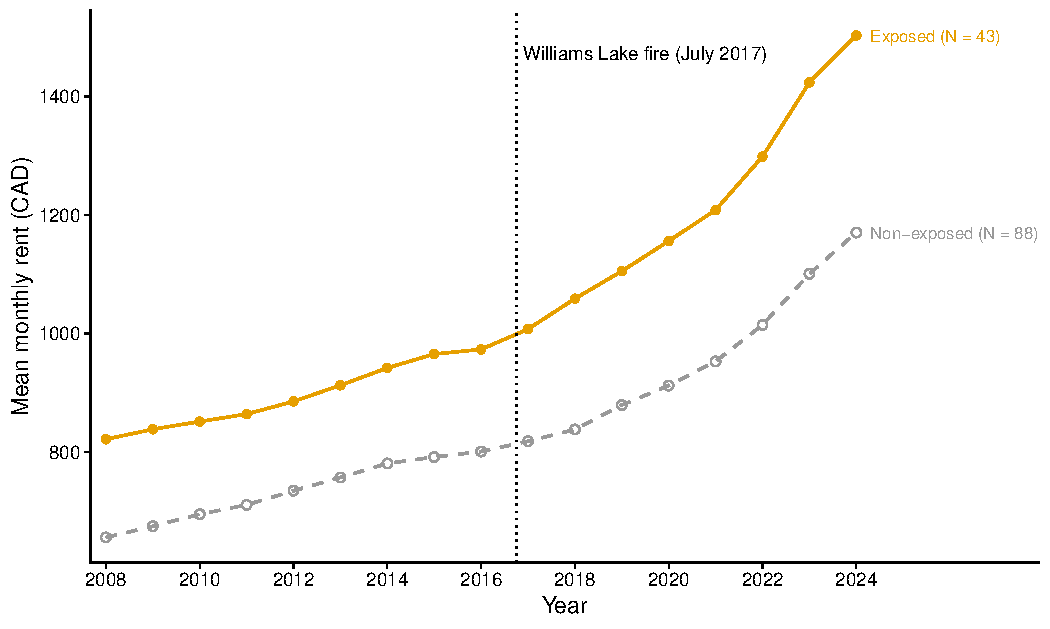
\includegraphics[width=0.78\textwidth]{figures/fig_rent_evolution}
  \par\smallskip\begin{minipage}{0.78\textwidth}\setstretch{1.0}\footnotesize\textit{Notes:} Annual cross-sectional mean of average monthly rent (CAD) for two-bedroom
    apartments in structures of three or more units, computed separately for
    exposed cities ($s_{WL,d}>0$, $N=43$, solid line) and non-exposed cities
    ($s_{WL,d}=0$, $N=88$, dashed line). The vertical dotted line marks 2017,
    the year of the Williams Lake wildfire.\end{minipage}
\end{figure}

% =============================================================================
% Ancien titre commenté : « Empirical Strategy » est plus standard en économie appliquée.
% \section{Empirical Design}
\section{Empirical Strategy}
\label{sec:strategy}

Two sources of variation drive the estimates. Across cities, some destinations
received a larger share of Williams Lake's pre-fire out-migrants than others,
for reasons tied to distance and labour-market proximity rather than to rental
conditions at the destination. Over time, the July~2017 evacuation activated
those pre-existing links. Cities with stronger historical ties to Williams Lake
faced a larger housing-demand shift from 2017 onward. The coefficient
$\hat\pi$ measures whether that differential exposure translated into faster
rent growth after 2017.

% Ancien titre commenté : trop explicatif ; le nouveau titre est plus académique.
% \subsection{Why a direct regression is unreliable}
\subsection{Endogeneity}

Estimating how wildfire-displaced households affect rents is harder than it
looks. Displaced households do not choose their destination at random: they move
toward cities where they have family ties, where labour markets are strong, or
where rents are already rising. This selective sorting creates a correlation
between observed migrant inflows and unmeasured characteristics of receiving
cities, so ordinary least squares estimates of the displacement effect would be
unreliable.

Selective sorting biases estimates in both directions. If displaced households move toward
dynamic cities whose rental prices are rising for reasons unrelated to the
wildfire, ordinary least squares will overstate the effect of displacement. If,
instead, they move toward cities perceived as relatively affordable, the same
correlation may bias estimates downward. In either case, the observed relation
between realised migration flows and rents does not by itself support a causal
interpretation.

Including city and year fixed effects partially mitigates this problem. City
fixed effects $\gamma_d$ absorb time-invariant differences in local housing
markets, geography, and amenities. Year fixed effects $\lambda_t$ absorb common
macroeconomic shocks affecting all Canadian cities. A two-way fixed-effects regression on observed inflows would take the form

\begin{equation*}
\log R_{dt} = \alpha + \beta M_{dt} + \gamma_d + \lambda_t + \varepsilon_{dt},
\end{equation*}

where $R_{dt}$ denotes the average monthly rent in city $d$ and year $t$, and
$M_{dt}$ denotes realised arrivals of displaced households. Even in this
framework, $M_{dt}$ may remain correlated with $\varepsilon_{dt}$ if
destination-specific shocks both attract migrants and raise rents. The empirical
strategy therefore replaces realised migration with a predetermined exposure
index based on pre-fire destination shares.

% Ancien titre commenté : trop long ; le nouveau titre isole le choc empirique.
% \subsection{The 2017 wildfire as the aggregate event}
\subsection{Wildfire Shock}

The institutional features of the Williams Lake evacuation reviewed in
Section~\ref{sec:wl_context} provide an aggregate event whose timing is
plausibly exogenous to rental-market conditions in potential receiving cities.
In the absence of the fire, migration flows between Williams Lake and the rest
of Canada would have followed their ordinary path, shaped by labour markets and
social networks. The wildfire created an abrupt evacuation shock that may have
been transmitted more strongly to cities with closer historical links to the
origin. The design exploits this cross-city variation in predetermined exposure
rather than realised post-fire mobility itself.

The pre-fire migration shares $s_{WL,d}$ are not distributed randomly across
Canadian cities. They reflect the economic geography of the British Columbia
Interior. Williams Lake, Quesnel, and Prince George lie along Highway~97, the
main north-south corridor of the province's forest economy, at intervals of
roughly 120--150~kilometres. Kamloops, 180~kilometres south of Williams Lake
via the same highway, is the largest regional service hub for the southern
Cariboo. West Fraser Timber and Canfor operate mills across this corridor,
creating overlapping labour markets: a mill worker from Williams Lake could
find equivalent employment in Quesnel or Prince George without changing
industry. When the evacuation order came, residents went to Kamloops, Prince
George, or Quesnel because they had worked in those cities before, had family
in the same industry there, or had simply driven through on prior occasions.
The shares measure this pre-existing economic geography. A gravity model fitted
directly to Williams Lake as origin, using destination population and bilateral
distance, explains $69$~percent of the cross-city variation in observed pre-fire
shares ($R^{2}=0.69$, Appendix Figure~\ref{fig:validation_wl}). Replacing observed
shares with these gravity-predicted counterparts yields similar main estimates
(Table~\ref{tab:soft_checks}, columns~2--3), confirming that $s_{WL,d}$ is driven by
observable economic fundamentals rather than idiosyncratic migration choices
correlated with destination rental markets.

% Ancien titre commenté : trop long et trop défensif.
% \subsection{A Bartik-style exposure index based on pre-fire migration links}
\subsection{Exposure Index}

The empirical design uses a Bartik-style exposure index rather than a canonical
multi-shock Bartik instrument. In the standard shift-share setting formalised
by \citet{goldsmith2020} and \citet{borusyak2022}, identification can be
organised around many independent shocks whose weighted sum varies across
locations. Here, the aggregate event is a single wildfire evacuation. Cross-city
variation comes entirely from one predetermined exposure profile: the pre-fire
destination shares of Williams Lake out-migrants. The relevant identifying
assumption is therefore not the exogeneity of a collection of shocks, but the
conditional exogeneity of these pre-fire shares, in the sense of
\citet{goldsmith2020}, with respect to destination-specific counterfactual
rent trajectories.

The migration share $s_{WL,d}$ is defined in equation~\eqref{eq:shares}. The
exposure variable interacts this predetermined cross-city share with a binary
post-treatment indicator:

\begin{equation}
Z_{WL,dt} = s_{WL,d} \times \mathbf{1}[t \geq 2017].
\label{eq:instrument}
\end{equation}

Before the wildfire, $Z_{WL,dt}=0$ for every city. From 2017 onward, a city's
exposure equals its pre-fire migration share $s_{WL,d}$. The 88 cities with
$s_{WL,d}=0$ serve as the low-exposure reference group in this reduced-form
design. They had no observed Williams Lake destination share in the pre-fire
wave, though the annual migration data do not justify treating them as receiving
literally zero displaced households after the evacuation. This cross-city
heterogeneity in exposure intensity, combined with temporal activation at the
moment of the shock, supplies the variation used in the main specification.
Because the wildfire is a single event shared by all destinations, the shift
component $\mathbf{1}[t \geq 2017]$ is constant across cities. All cross-city
variation in $Z_{WL,dt}$ therefore comes from the share component $s_{WL,d}$
alone.

The economic interpretation of the exposure index rests on a proportional
amplification idea. Cities that historically received a larger share of Williams
Lake out-migrants would face proportionally higher exposure to any wildfire-induced
relocation shock. Section~\ref{sec:channel} tests this reading directly
against the annual bilateral migration data. High-share destinations do not
record the post-fire surge in annual arrivals that a direct displacement
interpretation would predict. This negative result does
not invalidate the exposure index. Emergency evacuations unfold over days or weeks,
while the administrative migration series aggregates flows over twelve-month
windows. The displacement signal is too brief and too diffuse to register cleanly
in annual records. The exposure index is therefore best understood not as a proxy
for an observable flow that happens to be poorly measured, but as a predetermined
indirect measure of a process that leaves no clean administrative trace at the
available data frequency.

% Ancien titre commenté : formulation correcte mais moins sobre.
% \subsection{Econometric specification}
\subsection{Specification}

% ============================================================
% PRÉ-ENREGISTREMENT — EXPLICATION ET STATUT (pour la soutenance et les soumissions futures)
%
% QU'EST-CE QUE LE PRÉ-ENREGISTREMENT ?
% Avant de collecter ou d'analyser des données, un chercheur dépose publiquement
% un document précisant : quelle hypothèse il teste, quelles données il utilisera,
% quelle spécification empirique il emploiera. La plateforme standard en économie
% est l'AEA RCT Registry (https://www.socialscienceregistry.org/).
%
% POURQUOI LE FAIT-ON ?
% Sans pré-enregistrement, un lecteur ne peut pas savoir si l'auteur a testé
% 50 spécifications et n'a présenté que celle qui "marchait" (p-hacking ou
% specification mining). Le pré-enregistrement rend transparent le fait que
% les résultats n'ont pas été fabriqués après avoir regardé les données.
% Pour les ECR (expériences contrôlées randomisées), il est quasi-obligatoire.
% Pour les études observationnelles comme celle-ci, il reste recommandé.
%
% STATUT POUR CE MÉMOIRE :
% Cette étude N'a PAS été pré-enregistrée. Elle est purement observationnelle
% (pas d'intervention, pas d'assignation aléatoire). La spécification principale
% a été fixée avant estimation, mais aucun plan d'analyse préalable n'a été
% déposé sur l'AEA RCT Registry ou une plateforme équivalente.
%
% SI ON SOUMETTAIT À L'AER :
% Il faudrait ajouter une note de bas de page dans §4 :
%   "This study was not pre-registered. The empirical specification
%    was fixed before estimation, but no pre-analysis plan was filed."
% ============================================================
The main reduced-form specification regresses log rent on the exposure index $Z_{WL,dt}$ in equation~\eqref{eq:instrument}, with city and year fixed effects:\footnote{The decomposition concerns of \citet{goodman-bacon2021} and the estimator proposed by \citet{callaway2021} address staggered binary treatment adoption. This design involves a single simultaneous shock: all cities transition from pre-fire to post-fire exposure at the same calendar date (2017). Those critiques do not apply here. A related concern for \emph{continuous} treatments is that the two-way fixed effects estimator may assign negative weights to some average treatment effects when those effects are heterogeneous across intensities \citep{dechaisemartin2020}. For $Z_{WL,dt}=s_{WL,d}\times\mathbf{1}[t\geq 2017]$, the Frisch-Waugh-Lovell decomposition yields TWFE weights proportional to $(s_{WL,d}-\bar{s})^{2}\times(\mathrm{Post}_{t}-T^{\mathrm{post}}/T)^{2}\geq 0$ for all $(d,t)$. The simultaneous shock and time-invariant post-treatment intensity guarantee non-negative weights by construction; see Appendix~\ref{app:twfe_weights}.}

\begin{equation}
\log R_{dt} = \alpha + \pi Z_{WL,dt} + \gamma_d + \lambda_t + \varepsilon_{dt},
\label{eq:main}
\end{equation}

% AUDIT CLUSTERING (2026-05-19) — PASS
% Règle : "Cluster standard errors at the level of treatment or the level of
% potential serial correlation."
%
% Choix retenu : clustering ville (name_cancensus), justifié sur deux arguments :
%   (1) NIVEAU DU TRAITEMENT : s_{WL,d} est constant dans le temps et varie
%       uniquement entre villes. Le traitement est donc assigné à la ville.
%   (2) CORRÉLATION SÉRIELLE : les loyers d'une même ville sont corrélés
%       d'une année sur l'autre (chocs de demande et d'offre locaux persistants).
% Les deux arguments convergent vers le même niveau → clustering ville correct.
%
% ROBUSTESSE : Appendix Table tab:robustness_clustering confirme que le
% two-way clustering ville x province ne change pas les conclusions.
%
% NOTE MÉTHODOLOGIQUE (pour la soutenance) :
% Adão, Kolesár et Morales (2019, QJE, "Shift-Share Designs: Theory and
% Inference", vol. 134(4), pp. 1949-2010) montrent que dans les designs
% Bartik multi-secteurs, les erreurs-types clustérisées à la région peuvent
% être sous-estimées si les shares sont corrélées entre destinations (parce
% que chaque destination est exposée aux mêmes tendances nationales par
% industrie). Ils proposent une correction AKM. Dans notre cas à UNE SEULE
% ORIGINE (Williams Lake), la source de corrélation inter-destinations est
% structurellement différente et plus limitée : les shares s_{WL,d} reflètent
% la géographie migratoire d'une seule ville, pas des tendances nationales
% sectorielles. Le clustering ville reste donc le meilleur choix disponible
% et est conforme à la règle de base. Le two-way clustering province x ville
% en annexe couvre le cas où des chocs provinciaux induiraient une corrélation
% résiduelle entre villes de la même province.
\enlargethispage{3\baselineskip}
where $\gamma_d$ denotes city fixed effects and $\lambda_t$ denotes year fixed
effects. Standard errors are clustered at the city level to account for serial
correlation within destinations.\footnote{Adão, Kolesár, and Morales (2019) show that city-clustered standard errors can be understated in
multi-sector Bartik designs when shares are correlated across destinations
through common national trends. That concern is structurally limited here:
the shares $s_{WL,d}$ reflect the migration geography of a single origin city,
not exposure to national sectoral shocks. Two-way clustering by city and
province in Appendix Table~\ref{tab:robustness_clustering} covers the residual
case in which provincial shocks induce cross-city correlation.}
Appendix Table~\ref{tab:robustness_clustering}
verifies that two-way clustering at the city and province levels does not
materially alter inference. The coefficient $\pi$ measures the post-2017
log-rent differential associated with a one-unit increase in the exposure index.
Because no city has $s_{WL,d}=1$, the economically meaningful objects are
effects evaluated over the support of the observed exposure distribution, such
as a ten-percentage-point increase in exposure or the share observed for
Kamloops.

% ============================================================
% AUDIT CONTRÔLES — 2026-05-19
% Il n'y a aucune variable de contrôle additionnelle au-delà des effets fixes
% ville et année. Pas de kitchen sink. Les specs alternatives ajoutent des
% tendances linéaires par ville ($\delta_d \cdot t$) ou des effets fixes
% province$\times$année et région$\times$année --- des absorptions structurelles,
% pas des contrôles potentiellement endogènes.
%
% En particulier : on ne contrôle à aucun moment pour les taux de vacance
% post-2017, la construction neuve, les salaires locaux, ou tout autre
% déterminant de la demande de logement qui pourrait avoir été affecté par
% les évacués. C'est la bonne décision. Le coefficient $\hat\pi$ capte
% l'effet total du choc sur les loyers, sans bloquer les canaux intermédiaires.
% ============================================================
The error term $\varepsilon_{dt}$ captures city-specific shocks to rental
demand and supply that are not removed by city or year fixed effects. Several
forces belong there. British Columbia housing policies introduced during the
sample period (the Foreign Buyers Tax on Metro Vancouver purchases in
August~2016, the Speculation and Vacancy Tax announced in 2018) diverted
real-estate demand toward the rental market in ways that affected exposed and
unexposed cities differently. Commodity price cycles, particularly the oil
boom of 2012--2014 and the subsequent bust, generated income shocks for
resource-sector workers across the Interior that are not fully absorbed by
common year effects. The COVID-19 pandemic accelerated urban-to-secondary-city
migration after 2020, disproportionately toward the British Columbia cities
that also happen to be most exposed to Williams Lake migration links. Each of
these forces is a plausible source of differential rent growth between
high-exposure and low-exposure cities, independent of the 2017 wildfire. The
identification threat they pose is real and is confronted directly in
Section~\ref{sec:threats}.

The reduced form is the appropriate estimand given the observability structure of
the data. Because emergency displacement is not recorded at the frequency
required for a credible first stage, treating the exposure index as an instrument
for observed annual inflows would impose a mapping between the predetermined
network measure and an endogenous regressor that the data cannot validate.
Appendix Section~\ref{sec:appendix_iv} presents an exploratory fixed-effects
2SLS exercise.
The first stage is precisely estimated but negative,
reflecting mean reversion in annual flows rather than displacement amplification.
The reduced form avoids this mismatch by asking whether
cities with higher predetermined exposure exhibit different post-2017 rent paths,
without requiring that the displacement channel be directly observed at annual
frequency. I therefore do not interpret $\pi$ as a structural elasticity of rents
with respect to realised displaced arrivals.

A second specification adds city-specific linear trends to absorb pre-existing rent trajectories:

\begin{equation}
\log R_{dt} = \alpha + \pi Z_{WL,dt} + \gamma_d + \lambda_t
+ \delta_d \cdot t + \varepsilon_{dt}.
\label{eq:trends}
\end{equation}

This specification allows each city to follow its own linear rent trajectory
over the full sample. The exposure
profile is heavily concentrated in British Columbia, where rents were already
growing faster than the Canadian average before the wildfire. The city-trend
specification partially absorbs these pre-existing trajectories, but it does so
by requiring city-level counterfactual rents to be well approximated by linear trends. The estimates with and without city trends
are therefore reported as sensitivity benchmarks, not as endpoints of a formal
causal interval.

This is a reduced-form exposure specification. The coefficient $\pi$ is estimated
by least squares, but the object of interest is not an OLS regression of rents on
realised migration inflows. It is the post-2017 rent differential associated with
predetermined Williams Lake exposure, after absorbing permanent city differences
and common year shocks.
% Ancien titre commenté : trop défensif ; le contenu expliquera les menaces.
% \subsection{Identification challenges and threats to validity}
\subsection{Identification}
\label{sec:threats}

The Bartik-style exposure design rests on three distinct conditions: (i) the wildfire
itself must be exogenous to rental-market conditions in receiving cities, (ii) the
pre-fire migration shares $s_{WL,d}$ must be orthogonal to counterfactual rent
trajectories conditional on the absorbed fixed effects, and (iii) the wildfire must
activate the pre-existing exposure profile in a way that is economically relevant
for destination rental markets. The first condition is supported by the
meteorological nature and emergency timing of the event. The second and third
conditions are substantive identifying assumptions whose plausibility is
evaluated empirically.

Exogeneity of the aggregate wildfire shock does not by itself make the
cross-city exposure profile valid. The deeper problem is that the shares
$s_{WL,d}$ are high in British Columbia cities, which were already experiencing
faster rent growth than the Canadian average well before 2017. Asking whether cities with stronger Williams Lake ties saw higher
rent growth after 2017 is, to a significant degree, asking whether British
Columbia cities saw higher rent growth after 2017. They did, and the wildfire
is not why. Foreign investment pressure, zoning constraints, a booming tech
sector in Vancouver, and net in-migration from other provinces all drove British Columbia
rents upward during the same period. The pre-fire migration shares happen to
be correlated with this provincial trend, not because Williams Lake evacuees
caused it, but because the same economic geography that made certain cities
attractive destinations for Williams Lake migrants also made them attractive
to everyone else. The placebo tests in Section~\ref{sec:robustness} confirm
this reading. Re-estimating the baseline with fictitious treatment years
$\tau\in\{2010,\ldots,2016\}$ produces positive coefficients in most years,
meaning the data reject unconditional parallel trends. This is not a
routine diagnostic that the design comfortably passes. It is direct evidence
that the shares predict rent growth before the fire.

City-specific linear trends in equation~\eqref{eq:trends} absorb part of these
pre-existing trajectories, but only under the assumption that counterfactual
rents would have continued along a linear path. Province-year fixed effects,
which compare only cities within the same province and year, are more demanding.
They eliminate the British Columbia-versus-Canada confound directly, at the cost of absorbing
any within-province variation that genuinely reflects wildfire exposure.
The interpretation of the baseline estimate therefore turns on how much of the
post-2017 differential survives once regional rental-market dynamics are absorbed.

% ============================================================
% COMPOSITION SOCIO-DÉMOGRAPHIQUE — MENACE RÉSIDUELLE (2026-05-19)
%
% Ce n'est pas un défaut rédhibitoire. Le design avec effets fixes ville
% absorbe les différences de composition time-invariantes entre villes.
% Mais un referee pointilleux pourrait demander si la composition des ménages
% locataires dans les villes très exposées a évolué DIFFÉREMMENT post-2017
% (ex: afflux de nouveaux ménages à revenus plus élevés attirés pour des
% raisons autres que le feu). Ce serait un biais de composition time-varying.
%
% RÉPONSE DÉFENSIVE (pour la soutenance) :
%   (1) Les effets fixes ville absorbent la composition time-invariante.
%   (2) La tendance BC-wide est absorbée par les province×year FEs.
%   (3) C'est exactement pourquoi le province×year FE est le test le plus
%       exigeant : il compare des villes DANS la même province, où les
%       dynamiques de composition BC auraient joué de façon similaire.
%
% PEUT-ON TESTER CELA AVEC DES DONNÉES GRATUITES/PUBLIQUES ?
%   OUI, partiellement. Deux sources disponibles sans coût :
%
%   (A) Census 2016 + Census 2021 (PUMF = Public Use Microdata Files)
%       — Disponibles gratuitement via StatCan après inscription.
%       — Contiennent : tenure (propriétaire/locataire), revenu ménage,
%         statut de récent déménageur, CMA/CA code.
%       — On pourrait faire un DiD 2×2 :
%         Dep var = revenu moyen des locataires (ou % locataires) par ville
%         Traitement = s_{WL,d} × Post2021
%       — LIMITE MAJEURE : seulement 2 points temporels (2016 = pré-feu,
%         2021 = post-feu MAIS aussi post-COVID). Impossible de séparer
%         l'effet du feu de celui de COVID sur la composition.
%       — Résultat : exercice descriptif mais pas identification causale.
%
%   (B) Canadian Income Survey (CIS) annuelle via StatCan
%       — Données annuelles de revenu au niveau CMA mais échantillons
%         petits pour les 131 villes — bruit très élevé.
%
%   CONCLUSION : Techniquement faisable avec Census 2016+2021 PUMF,
%   mais la période post-traitement est contaminée par COVID → résultat
%   non interprétatble causalement. Mieux présenté comme "future research"
%   dans la conclusion plutôt que comme robustesse dans le papier actuel.
% ============================================================

The timing of the annual rent series creates a second, more mechanical
measurement issue. The wildfire occurred in July~2017, while the Canada Mortgage and Housing Corporation rent
series is observed at the annual frequency. Coding $\mathbf{1}[t\geq 2017]$ as
the post-treatment indicator assigns the 2017 observation to the exposed period
even though rental adjustment may be partial in the first calendar year. The
event-study coefficient at $k=0$ is small and not significant at conventional
levels, which is consistent with this timing issue and with lease-based frictions
in rent adjustment. Section~\ref{sec:robustness} therefore re-estimates the
baseline specification using $\mathbf{1}[t\geq 2018]$ as a direct timing check.

The estimand is reduced form by design, not by default. The variable $Z_{WL,dt}$
is not the realised number of displaced households entering city~$d$. It is a
predetermined index of exposure built from historical origin-destination shares.
Converting $\pi$ into a structural elasticity would require observing the
displacement flow itself at the relevant frequency, which the available data
do not permit. The reduced form sidesteps this unobservability
constraint by asking whether cities with stronger predetermined migration links
to a disaster origin exhibit systematically different rent trajectories after
the disaster. The coefficient $\pi$ measures
this post-2017 rent differential directly. Section~\ref{sec:channel} examines
whether annual bilateral migration flows independently corroborate the
displacement reading. Where that corroboration is absent, the interpretation
rests on the reduced-form pattern itself.

Taken together, these diagnostics define the scope of the research design. The
wildfire supplies plausibly exogenous timing, the pre-fire shares supply
predetermined cross-city exposure, and the coefficient $\pi$ measures a
reduced-form rent differential along that exposure profile. The design does not
claim to recover a structural elasticity of rents with respect to realised
displaced arrivals.
% =============================================================================
% Ancien titre commenté : trop long ; la version courte sonne davantage article.
% \section{The Migration Channel in Annual Bilateral Flows}
\FloatBarrier

\section{Migration Evidence}
\label{sec:channel}

The rent estimates use a predetermined exposure profile, not observed post-fire
migration. The available panel of annual city-to-city flows therefore provides a diagnostic
check, not a formal instrument for observed inflows. If the displacement channel
operates as the design assumes, destinations with larger pre-fire Williams Lake
shares should record systematically larger post-fire annual arrivals from Williams
Lake. Table~\ref{tab:channel_validation} formally tests this prediction. The answer is
negative. High-share destinations do not display the post-fire amplification
predicted by a direct annual-flow reading of the displacement channel.Appendix Figure~\ref{fig:migration_event_studies} reports the corresponding dynamic
profiles.

\begin{table}[tbp]
  \caption{Annual Migration-Flow Diagnostics}
  \label{tab:channel_validation}
  \centering
  \resizebox{\textwidth}{!}{%
  \begin{threeparttable}\small
    \begin{tabular}{lrr}
      \toprule
      \multicolumn{3}{l}{\textit{Dependent variable: bilateral annual migration arrivals from origin city. OLS.}} \\
      \addlinespace
      & (1) & (2) \\
      & Williams Lake & Placebo Quesnel \\
      \midrule
      WL migration share $\times$ Post-fire
                              & $-95.8^{***}$ & \\
                              & (8.9)    & \\
      \addlinespace
      Quesnel share $\times$ Post-fire
                              &          & 30.6 \\
                              &          & (29.5) \\
      \addlinespace
      Observations            & 655      & 655 \\
      R$^{2}$                 & 0.97     & 0.98 \\
      Within R$^{2}$          & 0.12     & 0.02 \\
      RMSE                    & 2.84     & 2.45 \\      \addlinespace
      Wave FE                 & $\checkmark$ & $\checkmark$ \\
      Destination FE          & $\checkmark$ & $\checkmark$ \\
      \bottomrule
    \end{tabular}
    \begin{tablenotes}[flushleft]\footnotesize
      \item \textit{Notes:} Each column reports a separate OLS regression of
        annual bilateral migration arrivals from the origin city to each
        destination city in the balanced rental-market sample.
        Column~(1): origin is Williams Lake; column~(2): origin is Quesnel
        (placebo). Post-fire is an indicator equal to one for migration waves
        2017/2018 onward; pre-fire wave: 2016/2017.
        Standard errors clustered at the destination city level in parentheses.
        Wave FE: fixed effects for Statistics Canada annual migration waves
        (July--June periods), distinct from the calendar-year fixed effects
        used in the rent regressions.
        * $p < 0.10$, ** $p < 0.05$, *** $p < 0.01$.
    \end{tablenotes}
  \end{threeparttable}}
\end{table}

This result limits interpretation. Annual migration records may miss short-lived
emergency relocations, and the same pre-fire wave used to define shares can make
post-period comparisons prone to a statistical pull toward the average. Even so, the flow
data do not directly validate the channel that motivates the exposure design.
The rent estimates therefore remain reduced form, documenting a post-2017
rental-market pattern aligned with pre-fire Williams Lake links without
establishing that realised displaced inflows are the sole mechanism.

% =============================================================================
% Ancien titre commenté : trop explicatif ; le nouveau titre est plus net.
% \section{Main Effects on Rental Prices}
\section{Rental Effects}
\label{sec:results}

The baseline reduced-form estimate is $\hat{\pi} = 0.818$
(s.e.\ $0.216$). For Kamloops, the most exposed destination with
$s_{WL,d} = 0.212$, this point estimate implies a post-2017 rent differential
of approximately $19$~percent relative to an unexposed city. At the 2015
national reference rent of \$848, that translates to roughly \$160~per month on average over the post-2017 period.
% OPTION EDITORIALE (AER audit) : ajouter une phrase sur l'IC du baseline pour
% formuler un "rule out" explicite. Exemple :
% "The 95~percent confidence interval for the baseline estimate runs from
% approximately $0.39$ to $1.25$, ruling out effects smaller than roughly
% 4~percent for Kamloops at the sample mean exposure."
% Conservé en commentaire : la discussion économique (\$160/mois, 19\%)
% est jugée suffisante pour le corps du texte.
All estimates in this section are reduced-form, so $\hat{\pi}$ captures the
conditional association between pre-fire exposure and post-2017 rent
trajectories rather than a structural causal effect. Section~\ref{sec:channel} showed
that annual migration flows do not validate the displacement channel directly,
so the coefficient should be read as a network-correlation pattern, not a clean
causal estimate.

% Ancien titre commenté : simple correction de style.
% \subsection{Main results}
\subsection{Main Estimates}

Figure~\ref{fig:scatter_reducedform} provides the cross-sectional intuition
directly. Cities with larger pre-fire Williams Lake migration shares show
larger post-2017 rent increases after removing year effects. The slope of
that relationship is $\hat{\pi} = 0.818$.
Table~\ref{tab:main_result} breaks this down across five specifications.

The raw data already hint at the pattern. Panel~B of Table~\ref{tab:desc_stats}
shows that exposed cities saw average monthly rents rise from \$895 to \$1{,}219
between the pre-2017 and post-2017 periods, a $36$~percent increase.
Non-exposed cities grew from \$733 to \$961, or $31$~percent. That
5-percentage-point unconditional gap requires no fixed effects. It is simply in
the means. The fixed-effects specification tightens this comparison
by holding constant permanent city differences and common national trends, and
it exploits the continuous variation in exposure shares rather than a binary split. The
reduced-form estimate of $0.818$ is the residual association once those
confounds are absorbed.

The column-by-column pattern in Table~\ref{tab:main_result} shows how much of
the raw gap is explained by permanent city differences and common national
trends. The no-fixed-effects estimate estimate of $3.84$ $(1.05)$ picks up the
structural expensiveness of British Columbia cities. Year fixed effects bring it to $2.49$.
City fixed effects alone yield $3.40$. The two-way specification absorbs both,
and the coefficient falls to $0.818$ $(0.216)$. Adding city-specific linear
trends reduces it further to $0.594$ $(0.175)$. The two estimates bracket the
result from opposite directions.

% =============================================================================
% FIGURE 3 — page 28
% =============================================================================
\begin{figure}[H]
  \centering\singlespacing
  \caption{Reduced-Form Relationship: Pre-Fire Exposure and Post-2017 Rent Changes}
  \label{fig:scatter_reducedform}
  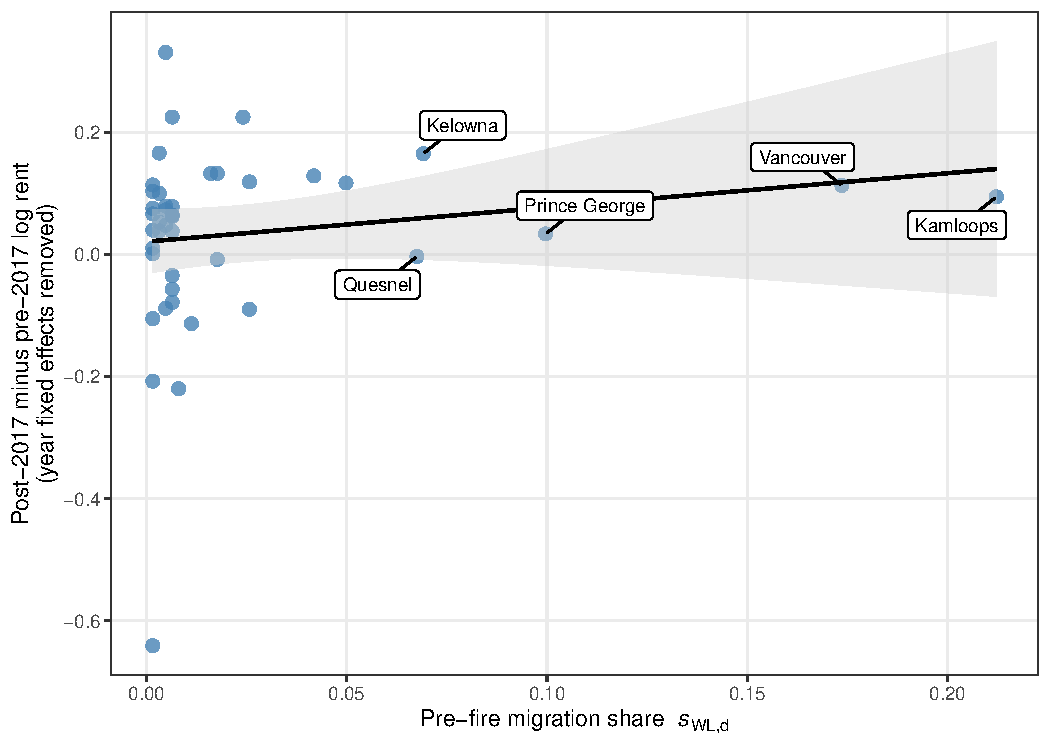
\includegraphics[width=0.78\textwidth]{figures/scatter_reducedform}
  \par\smallskip\begin{minipage}{0.78\textwidth}\setstretch{1.0}\footnotesize\textit{Notes:} Each point is an exposed city ($s_{WL,d}>0$, $N=43$). The $x$-axis plots
    the pre-fire Williams Lake migration share $s_{WL,d}$ (in decimal units);
    the $y$-axis plots the post-minus-pre change in log monthly rent (log points)
    after removing year fixed effects. The solid line shows the least-squares fit of the reduced-form exposure
relationship. The five most exposed destinations are labelled.\end{minipage}
\end{figure}

% =============================================================================
% TABLE 3 — top of page 29
% =============================================================================
\begin{table}[!htbp]
  \centering
  \caption{Reduced-Form Rent Effects by Williams Lake Exposure}
  \label{tab:main_result}
  \small

  \resizebox{\textwidth}{!}{%
  \begin{tabular}{lccccc}
    \toprule
    & (1) & (2) & (3) & (4) & (5) \\
    & No FE & Year FE & City FE & City + Year FE & City Trends \\
    \midrule
    WL exposure index
      & 3.838$^{***}$ & 2.488$^{***}$ & 3.397$^{***}$ & 0.818$^{***}$ & 0.594$^{***}$ \\
      & (1.050) & (0.856) & (0.848) & (0.216) & (0.175) \\
    \addlinespace
    Observations & 2{,}225 & 2{,}225 & 2{,}225 & 2{,}225 & 2{,}225 \\
    $R^{2}$      & 0.06 & 0.32 & 0.66 & 0.94 & 0.98 \\
    Within $R^{2}$ & & 0.03 & 0.07 & 0.02 & 0.01 \\
    RMSE         & 0.300 & 0.254 & 0.179 & 0.075 & 0.049 \\
    \addlinespace
    Year FE      &        & $\checkmark$ &        & $\checkmark$ & $\checkmark$ \\
    City FE      &        &              & $\checkmark$ & $\checkmark$ & $\checkmark$ \\
    City trends  &        &              &        &              & $\checkmark$ \\
    \bottomrule
  \end{tabular}
  }

  \par\smallskip
  \begin{minipage}{0.96\textwidth}
  \setstretch{1.0}
  \footnotesize
  \textit{Notes:} This table reports reduced-form exposure estimates. The dependent
  variable is log monthly rent for two-bedroom apartments in buildings with at
  least three units. The Williams Lake exposure index is the predetermined
  pre-fire destination share $s_{WL,d}$ interacted with a post-2017 indicator.
  Column~(5) includes city-specific linear time trends. Standard errors are
  clustered at the city level in parentheses. Period: 2008--2024.
  * $p<0.10$, ** $p<0.05$, *** $p<0.01$.
  \end{minipage}
\end{table}
% Ancien titre commenté : trop long ; les pré-tendances restent discutées dans le texte.
% \subsection{Dynamic effects and pre-trend diagnostics}
\FloatBarrier

\subsection{Dynamics}
\label{sec:event_study}

The July 2017 evacuation order reached Williams Lake residents with less than
24~hours of warning, providing a sharp demand shock to the migration networks
documented in Section~\ref{sec:data}. Figure~\ref{fig:event_study_wl} tracks
how rents in connected cities evolved year by year relative to 2016.
Each coefficient $\hat{\beta}_k$ comes from a fully interacted specification
that regresses log rent on $s_{WL,d}\times\mathbf{1}[\text{year}=2017+k]$,
with city and year fixed effects and the final pre-fire year $k=-1$ omitted
as the reference period.

% =============================================================================
% FIGURE -- RENT EVENT STUDY
% =============================================================================
\begin{figure}[t]
  \centering\singlespacing
  \caption{Event Study: Williams Lake Exposure and Rental Prices}
  \label{fig:event_study_wl}
  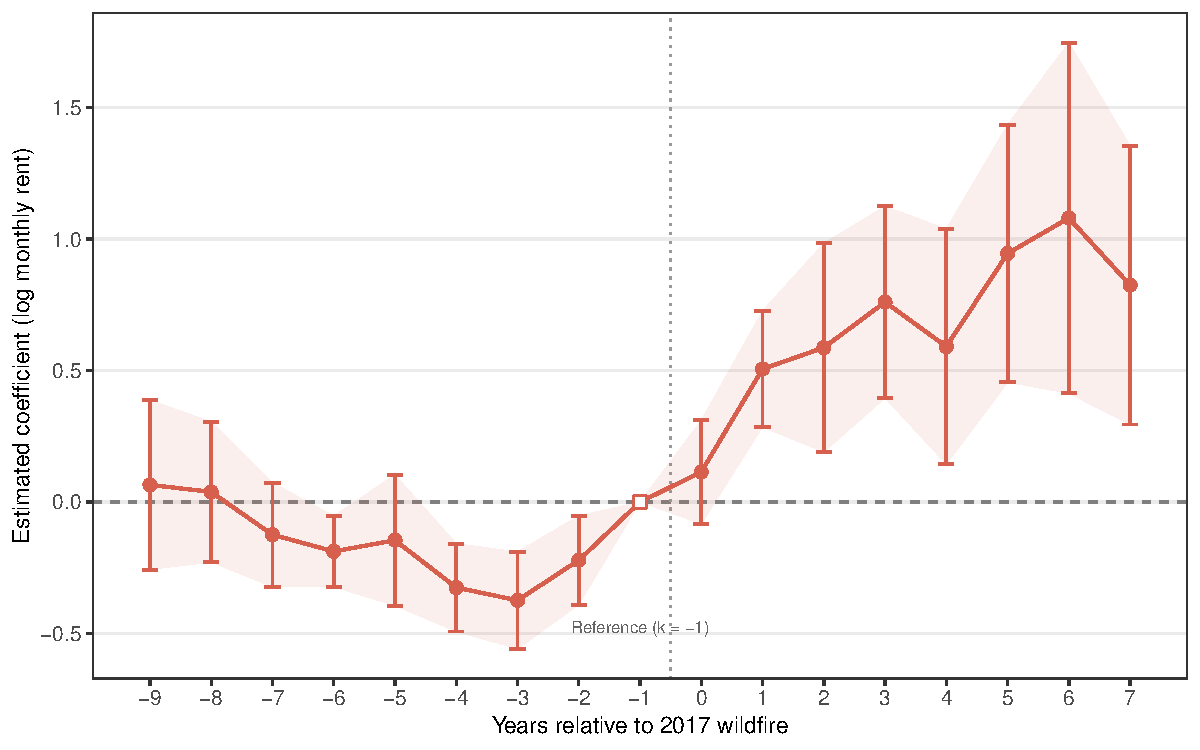
\includegraphics[width=0.82\textwidth,page=1]{figures/event_study_wl_pretrends}
  \par\smallskip\begin{minipage}{0.82\textwidth}\setstretch{1.0}\footnotesize\textit{Notes:} Coefficients $\hat{\beta}_k$ from a fully interacted specification that
    regresses log rent on
    $s_{WL,d}\times\mathbf{1}[\mathrm{year}=2017+k]$, with city and year fixed
    effects. The omitted reference year is 2016 ($k=-1$). Shaded bands denote
    95\% confidence intervals. Standard errors are clustered at the city level.
    Dependent variable: log monthly rent for two-bedroom apartments in buildings
    with at least three units. Period: 2008--2024.\end{minipage}
\end{figure}

The pre-treatment coefficients for $k\in\{-9,\ldots,-2\}$ are negative in
several periods and some confidence intervals exclude zero (the largest
deviation in absolute value is $\hat{\beta}_{-3}=-0.374$ at $k=-3$,
s.e.\ $0.094$). The pattern shows no monotonic divergence toward higher
rents before 2017. The most plausible
interpretation is that 2016, the reference year, coincided with a province-wide rent
acceleration that makes earlier years appear relatively lower for exposed cities
when measured against that baseline. The event study examines year-specific
deviations relative to 2016, whereas the placebo-treatment design in
Section~\ref{sec:robustness} tests whether the cumulative binary jump
structure falsely detects effects in earlier years. These diagnostics target
different objects and are both informative. Anticipation effects are
implausible in this setting. The evacuation order was issued with less than
24~hours of notice, leaving no window for property owners or tenants in
receiving cities to price in the shock in advance.

The coefficient at $k=0$ is $0.256$ (s.e.\ $0.162$), with a 95~percent
confidence interval of $[-0.062,\;0.574]$. This is an imprecise null rather than a precisely estimated zero, as the
upper bound of the interval reaches values comparable to those observed
at $k=2$ and beyond. The most likely mechanical
explanation is that Canada Mortgage and Housing Corporation measures rents in
October, three months after the July wildfire, so lease-based adjustment
would not be complete within a single calendar year. From $k=1$ onward,
coefficients grow and remain positive, with $\hat{\beta}_1=0.648$ (s.e.\ $0.150$),
$\hat{\beta}_3=0.902$ (s.e.\ $0.202$), and $\hat{\beta}_6=1.222$
(s.e.\ $0.348$; 95\% CI $[0.540,\;1.904]$). For Kamloops,
$\hat{\beta}_6$ implies a differential of roughly
$1.222\times0.212\approx0.259$ log-points, or about $29.5$~percent in levels,
relative to an unexposed city.

This dynamic pattern is compatible with a gradual receiving-market response,
but it is also compatible with the regional pre-trend concern identified in the
placebo tests. A one-time evacuation lasting approximately three weeks cannot
by itself explain rent differentials that persist and grow for seven years.
The post-2020 acceleration is partly attributable to COVID-era migration toward
British Columbia secondary cities, as confirmed by the truncation check in
Section~\ref{sec:angrist_checks}, which reduces the estimate from $0.818$
to $0.544$ when the sample is restricted to 2019. The event-study evidence
therefore strengthens the descriptive pattern, not the causal attribution.

% Ancien titre commenté : formulation trop longue.
% \subsection{Heterogeneity across rental-market segments}
\subsection{Segment Heterogeneity}

Displaced households arrive with different family compositions, from
single workers to families with children, so demand pressure from the
Williams Lake evacuation should not be confined to two-bedroom units.
The ex-ante prediction serves as a breadth check. If the two-bedroom baseline
reflects genuine market-wide pressure rather than a segment-specific
pricing pattern, comparable coefficients should appear across other
apartment types. Appendix Figure~\ref{fig:heterogeneity_coefplot}
confirms this. Positive coefficients of comparable magnitude appear
across the three well-covered segments. Row-house cells are too sparse
to carry weight. This breadth check does not address the paper's central
identification concern and is therefore reported in Appendix Figure~\ref{fig:heterogeneity_coefplot}.
% AUDIT VISUEL (2026-05-19) :
% Les tables tab:heterogeneity_size_region et tab:supply_het (7 sous-groupes
% au total : small/medium/large, West/East, tight/slack) ont été remplacées
% par un coefficient plot unique (fig:heterogeneity_all_dims) généré dans
% beta17.R section IX.7.3ter. Les tables restent en annexe pour la précision
% numérique mais le renvoi principal est désormais visuel.
To address multiple testing concerns, I examine four dimensions of heterogeneity in total, covering apartment
segment, city size, East-versus-West region, and housing supply
constraints following \citet{saiz2010}. Appendix Figure~\ref{fig:heterogeneity_all_dims}
plots the point estimates and 95\% confidence intervals across all
seven subgroups, visualizing the full set of cuts regardless of
significance. None contradicts the pooled estimate.

% Ancien titre commenté : « calibration » sonne technique ; le nouveau titre est plus lisible.
% \subsection{Economic calibration}
\subsection{Economic Magnitudes}
\label{sec:economic_calibration}

The reduced-form coefficients translate into city-level magnitudes through the
observed exposure shares (Table~\ref{tab:calibration}). Under the baseline
estimate $\hat{\pi}=0.818$, the implied log-rent differential, its percentage
equivalent, and its dollar equivalent appear in the first set of columns.
The final column repeats the calculation using the city-trend coefficient
$\hat{\pi}=0.594$. These values are scale conversions of the reduced-form
association, not estimates of a structural rent elasticity.

The same table also reports a deliberately simple potential-demand scenario. It
starts from the $11{,}000$ Williams Lake evacuees, allocates them across
destinations using the pre-fire exposure shares $s_{WL,d}$, assumes that a
fraction $q=0.25$ generates rental demand in receiving cities, and converts
persons into households using $h=2$ persons per unit. Under this illustrative
scenario, the implied number of renter households is approximately $292$ in
Kamloops, $239$ in Vancouver, $137$ in Prince George, $95$ in Kelowna, and
$93$ in Quesnel. These numbers are not realised flows and do not contradict the
negative annual-flow diagnostic in Section~\ref{sec:channel}. They provide only
an order-of-magnitude translation of the exposure profile into potential demand
counts.

\begin{table}[htbp]
  \caption{Economic Calibration of the Reduced-Form Magnitudes}
  \label{tab:calibration}
  \centering\small
  \resizebox{\textwidth}{!}{%
  \begin{threeparttable}
    \begin{tabular}{lrrrrrrr}
      \toprule
      City
        & Share\textsuperscript{a}
        & Displaced\textsuperscript{b}
        & Households\textsuperscript{c}
        & Log-point effect\textsuperscript{d}
        & $\Delta$\% baseline\textsuperscript{e}
        & $\Delta$\$ baseline\textsuperscript{f}
        & $\Delta$\% trend\textsuperscript{g} \\
      \midrule
      Kamloops      & 0.212 & 2{,}334 & 292 & 0.174 & 19.0 & 161 & 13.4 \\
      Vancouver     & 0.174 & 1{,}910 & 239 & 0.142 & 15.3 & 129 & 10.9 \\
      Prince George & 0.100 & 1{,}096 & 137 & 0.082 &  8.5 &  72 &  6.1 \\
      Kelowna       & 0.069 &     760 &  95 & 0.057 &  5.8 &  49 &  4.2 \\
      Quesnel       & 0.068 &     743 &  93 & 0.055 &  5.7 &  48 &  4.1 \\
      \bottomrule
    \end{tabular}
    \begin{tablenotes}[flushleft]\small\setstretch{1.0}
      \item \textit{Notes:} Top-five most exposed cities in the main sample.
        \textsuperscript{a}~$s_{WL,d}$: pre-fire Williams Lake migration share.
        \textsuperscript{b}~$11{,}000 \times s_{WL,d}$: evacuees allocated
        to city~$d$ under full dispersion.
        \textsuperscript{c}~Potential renter households under the illustrative
        scenario $(q,h)=(0.25,\,2)$:
        $\widehat{H}_{d}=q\times 11{,}000\times s_{WL,d}/h$.
        \textsuperscript{d}~$\hat{\pi}\times s_{WL,d}$ using
        $\hat{\pi}=0.818$ from column~(4) of Table~\ref{tab:main_result}.
        \textsuperscript{e}~$(\exp(\hat{\pi}\,s_{WL,d})-1)\times 100$.
        \textsuperscript{f}~$\Delta\%\times\$848$, the 2015 CMHC national average
        monthly rent (pre-fire reference, all 131 sample cities).
        \textsuperscript{g}~Same calculation using $\hat{\pi}=0.594$
        from column~(5) of Table~\ref{tab:main_result}.
        Household counts are scenarios, not estimates of realised
        post-fire relocations.
    \end{tablenotes}
  \end{threeparttable}}
\end{table}

Potential-demand counts can be compared with immediately available rental capacity
in each destination (Table~\ref{tab:vacancy_calibration}). For each
of the five most exposed cities, the table uses the October~2017 Canada Mortgage and Housing Corporation Rental
Market Survey count of private two-bedroom apartment units and the corresponding
two-bedroom vacancy rate. This segment closely matches this paper's main outcome.
Implied vacant units equal the two-bedroom rental universe multiplied by the
vacancy rate. The final columns report the ratio of potential renter households
to vacant two-bedroom apartment units under three scenarios:
$q=0.10$, $q=0.25$, and $q=0.50$, with $h=2$ in each case.

\begin{table}[htbp]
  \caption{Potential Rental Demand Relative to Vacant Two-Bedroom Apartments in 2017}
  \label{tab:vacancy_calibration}
  \centering\small
  \begin{threeparttable}
    \resizebox{\textwidth}{!}{%
    \begin{tabular}{lrrrr rrr}
      \toprule
      & & & Implied & &
        \multicolumn{3}{c}{Households / vacant units} \\
      \cmidrule(lr){6-8}
      City
        & Units\textsuperscript{a}
        & Vacancy\textsuperscript{a}
        & vacant
        & Households\textsuperscript{b}
        & $q=0.10$ & $q=0.25$ & $q=0.50$ \\
      \midrule
      Kamloops      & 1{,}499  & 1.1\% & 16.5  & 292  &  7.1 & 17.7 & 35.4 \\
      Vancouver     & 26{,}375 & 1.0\% & 263.8 & 239  &  0.4 &  0.9 &  1.8 \\
      Prince George & 1{,}505  & 3.0\% & 45.1  & 137  &  1.2 &  3.0 &  6.1 \\
      Kelowna       & 2{,}341  & 0.2\% & 4.7   &  95  &  8.1 & 20.3 & 40.6 \\
      Quesnel       & 318      & 3.0\% & 9.5   &  93  &  3.9 &  9.7 & 19.5 \\
      \bottomrule
    \end{tabular}}
    \begin{tablenotes}[flushleft]\footnotesize
      \item \textit{Notes:}
        \textsuperscript{a}~Two-bedroom units and vacancy rates from the
        Canada Mortgage and Housing Corporation (CMHC) 2017 British Columbia
        Rental Market Report, private apartment structures with at least three
        rental units, measured October~2017.
        Implied vacant units equal two-bedroom units multiplied by the
        vacancy rate.
        \textsuperscript{b}~Potential renter households under the
        intermediate scenario $(q,h)=(0.25,\,2)$ from
        Table~\ref{tab:calibration}.
        $H/V$ columns report potential renter households divided by implied
        vacant two-bedroom units under three scenarios for the share of
        evacuees generating rental demand ($q$), with household size $h=2$.
        This table is a market-tightness plausibility exercise, not an
        estimate of realised migration or a test of the identification
        strategy.
    \end{tablenotes}
  \end{threeparttable}
\end{table}

The ratios are large in small markets. Under the intermediate
scenario, potential renter households amount to roughly $18$ times the stock of
vacant two-bedroom apartments in Kamloops, about $20$ times in Kelowna, nearly
$10$ times in Quesnel, and about $3$ times in Prince George. Vancouver is the exception.
Its two-bedroom rental stock is large enough that the same scenario implies
a ratio below one. These calculations show that the reduced-form magnitudes are
not mechanically implausible for smaller, highly exposed markets that were
already very tight in October~2017. They do not establish that displaced
Williams Lake households generated the rent differentials estimated in
Section~\ref{sec:results}. Conversely, the large household-to-vacant-unit
ratios, reaching $17.7\times$ for Kamloops under the intermediate
scenario, suggest that a pure displacement channel operating through
standard market clearing would generate price pressures exceeding the
$19$~percent baseline estimate.Because the calibration starts from the roughly 11,000 Williams Lake evacuees
rather than the broader regional population affected by the 2017 wildfire season,
it should be interpreted as a conservative lower-bound scenario for potential
receiving-market demand, conditional on the displacement interpretation.

% =============================================================================
% Ancien titre commenté : trop long et défensif ; le contenu couvre déjà ces dimensions.
% \section{Robustness, Identification Diagnostics, and Interpretation}
\section{Robustness}
\label{sec:robustness}

This section focuses on the three diagnostics that matter most for
interpretation, covering pre-trend violations, regional confounding, and
the specificity of the Williams Lake exposure profile. Secondary checks are reported in Appendix Tables~\ref{tab:robustness_clustering} and~\ref{tab:robustness_instrument}.

% Ancien titre commenté : trop long ; le nouveau titre est plus direct.
% \subsection{Placebo treatment years and identification validity}
\subsection{Placebo Tests}
\label{sec:placebo_diagnostics}

The placebo treatment-year exercise is the central diagnostic for the baseline
design. For each fictitious treatment year
$\tau\in\{2010,\ldots,2016\}$, equation~\eqref{eq:main} is re-estimated after
replacing $\mathbf{1}[t\geq 2017]$ with $\mathbf{1}[t\geq \tau]$. If the
baseline coefficient were driven only by the post-2017 Williams Lake event,
these placebo exposures should not systematically predict rent growth before
the actual wildfire.

% =============================================================================
% FIGURE -- PLACEBO TESTS
% =============================================================================
\begin{figure}[t]
  \centering\singlespacing
  \caption{Placebo Treatment-Year Diagnostics}
  \label{fig:placebo}
  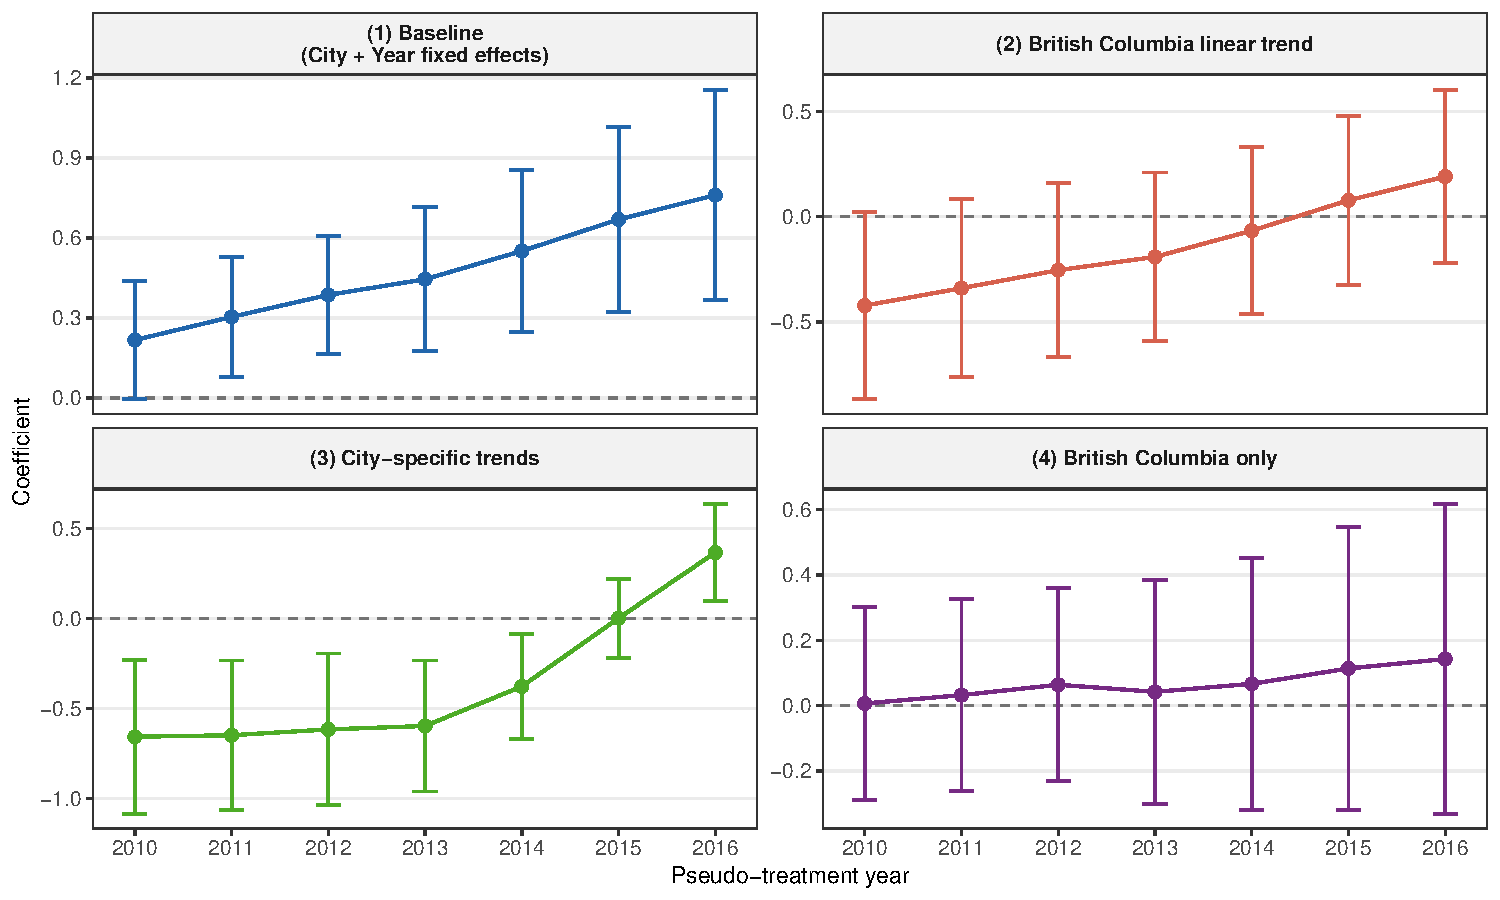
\includegraphics[width=0.85\textwidth]{figures/placebo_tests}
  \par\smallskip\begin{minipage}{0.85\textwidth}\setstretch{1.0}\footnotesize\textit{Notes:} Each panel plots the coefficient on
    $\tilde{Z}_{WL,dt}(\tau)=s_{WL,d}\times\mathbf{1}[t\geq \tau]$ for
    $\tau\in\{2010,\ldots,2016\}$. The panels correspond to:
    (i) city and year fixed effects,
    (ii) the baseline augmented with a British Columbia-specific linear trend,
    (iii) the baseline augmented with city-specific linear trends, and
    (iv) the British Columbia subsample. Bars show 95\% confidence intervals.
    Standard errors are clustered at the city level. Dependent variable: log
    monthly rent, two-bedroom apartments, buildings $\geq 3$ units. Period:
    2008--2024.\end{minipage}
\end{figure}

Figure~\ref{fig:placebo} shows that this implication fails in the baseline specification.
All seven placebo coefficients are positive, they become larger
as the fictitious treatment year approaches 2017, and most are statistically
distinguishable from zero. This pattern indicates that cities with greater
Williams Lake exposure were already on different rent trajectories before the
wildfire. Given the geographic concentration of exposure, the most plausible
reading is a British Columbia trend component correlated with the exposure
profile.

Additional controls partially attenuate the pre-trend imbalance but do not erase it.
Adding a British Columbia-specific linear trend makes the placebo coefficients
imprecise and reduces the main post-2017 coefficient to
$0.261$ $(0.214)$ in Table~\ref{tab:robustness_identification}. City-specific
linear trends also weaken the placebo pattern, but they rely on a stronger
functional-form assumption for the counterfactual rent path. Restricting the
sample to British Columbia does not reveal significant placebo coefficients, but
that subsample contains only 24 cities and therefore has limited power. The
appropriate conclusion is not that within-province parallel trends are established,
but that the strongest evidence of pre-trend imbalance operates across provinces.

The checks do not isolate a preferred estimate. The estimates in Table~\ref{tab:robustness_identification}
range from $0.144$ to $0.873$ across specifications, reflecting genuine uncertainty
about the counterfactual trend path.

% =============================================================================
% TABLE -- ROBUSTNESS: IDENTIFICATION CHECKS
% =============================================================================
\begin{landscape}
\begin{table}[htbp]
  \caption{Identification and Specification Checks}
  \label{tab:robustness_identification}
  \centering\small
  \begin{threeparttable}
    \begin{tabular}{lrrrrrrrr}
      \toprule
                                    & (1)           & (2)           & (3)          & (4)          & (5)      & (6)           & (7)           & (8)           \\
                                    & Baseline      & City trends   & BC trend     & Province trends& BC only  & Unbalanced    & WL+FM         & $t\geq 2018$  \\
      \midrule
      $Z_{WL}$                       & 0.818$^{***}$ & 0.594$^{***}$ & 0.261        & 0.298        & 0.144    & 0.828$^{***}$ & 0.835$^{***}$ & 0.873$^{***}$ \\
                                    & (0.216)       & (0.175)       & (0.214)      & (0.219)      & (0.260)  & (0.218)       & (0.234)       & (0.222)       \\[4pt]
      $Z_{FM}$                       &               &               &              &              &          &               & $-$0.670      &               \\
                                    &               &               &              &              &          &               & (0.813)       &               \\
      \midrule
      Observations   & 2{,}225      & 2{,}225       & 2{,}225      & 2{,}225      & 408      & 2{,}382       & 2{,}242       & 2{,}225       \\
      $R^{2}$        & 0.94         & 0.98          & 0.94         & 0.95         & 0.92     & 0.94          & 0.95          & 0.94          \\
      Within $R^{2}$ & 0.02         & 0.01          & 0.00         & 0.00         & 0.00     & 0.02          & 0.03          & 0.02          \\
      \midrule
      Year FE        & $\checkmark$ & $\checkmark$  & $\checkmark$ & $\checkmark$ & $\checkmark$ & $\checkmark$ & $\checkmark$ & $\checkmark$ \\
      City FE        & $\checkmark$ & $\checkmark$  & $\checkmark$ & $\checkmark$ & $\checkmark$ & $\checkmark$ & $\checkmark$ & $\checkmark$ \\
      City trend     &              & $\checkmark$  &              &              &          &               &               &               \\
      BC trend       &              &               & $\checkmark$ &              &          &               &               &               \\
      Province trend &              &               &              & $\checkmark$ &          &               &               &               \\
      \bottomrule
    \end{tabular}
    \begin{tablenotes}[flushleft]\footnotesize
      \item \textit{Notes:} Dependent variable: log monthly rent for
        two-bedroom apartments in buildings with at least three units.
        $Z_{WL}=s_{WL,d}\times\mathrm{Post}_{2017}$ is the Williams Lake
        Bartik exposure index. Column~(3) adds a British Columbia-specific linear time
        trend. Column~(4) adds province-specific linear time trends.
        Column~(5) restricts the sample to British Columbia cities
        ($N=408$ city-year observations). Column~(6) uses the unbalanced
        panel retaining all cities with at least one non-missing rent
        observation ($N=2{,}382$). Column~(7) adds $Z_{FM}$, the Fort
        McMurray exposure index based on gravity-predicted destination shares
        interacted with $\mathrm{Post}_{2016}$. Column~(8) replaces
        $\mathrm{Post}_{2017}$ with $\mathbf{1}[t\geq 2018]$. All
        specifications include city and year fixed effects. FE: fixed effects.
        Standard errors clustered at the city level in parentheses.
        Within $R^{2}=0.00$ in columns~(3)--(4) indicates that $Z_{WL}$
        explains no residual within-cell variation once province-specific
        or British Columbia linear trends are absorbed, consistent with
        the regional confounding hypothesis.
        Period: 2008--2024.
        * $p < 0.10$, ** $p < 0.05$, *** $p < 0.01$.
    \end{tablenotes}
  \end{threeparttable}
\end{table}
\end{landscape}

% Ancien titre commenté : formulation lourde pour la table des matières.
% \subsection{Sensitivity to parallel-trend violations}
\subsection{Trend Sensitivity}
\label{sec:rambachan_roth}

The placebo evidence motivates an explicit sensitivity analysis rather than a
binary accept-or-reject treatment of parallel trends.
Table~\ref{tab:rambachan_roth} in the Appendix implements the honest-inference
framework of \citet{rambachan2023}. The analysis asks how large post-treatment
deviations from parallel trends may be, relative to the largest observed
pre-treatment deviation, before the post-2017 rent differential can no longer be
distinguished from zero.

The breakdown value reported in the Appendix is $\bar{M}^{*}=0.38$. In
substantive terms, the post-2017 confidence set ceases to exclude zero once
future trend violations are allowed to reach roughly two-fifths of the largest
pre-treatment deviation. This is not a reassuring robustness margin. It
quantifies the same point made visually by the placebo plots. The rent pattern is
statistically sharp under the baseline specification, but its causal
interpretation is sensitive to modest departures from the identifying trend
restriction.

% Ancien titre commenté : trop technique ; le nouveau titre donne l'enjeu d'identification.
% \subsection{Regional absorption and exposure concentration}
\subsection{Regional Confounding}
\label{sec:prov_year_fe}

The central identification challenge is that nearly all exposed cities are located
in British Columbia, which experienced provincial rent growth systematically above
the Canadian average from 2010 onward. The province-by-year fixed effects
specification addresses this directly by comparing only cities within the same
province and calendar year, absorbing any province-level annual shock, including
the combined effect of British Columbia housing policies and broader demand dynamics documented
in Section~\ref{sec:bc_policy}. Under this specification, the coefficient falls
to $0.164$ $(0.260)$ (Table~\ref{tab:prov_year}, column~2). This is the most
important single number in the robustness analysis. The 95~percent confidence
interval runs from approximately $-0.35$ to $+0.49$, which spans both zero and
effects as large as the baseline estimate. This is not a precisely estimated
zero. The province-year specification absorbs most of the identifying variation
with only 24 British Columbia cities in the sample, so the test cannot rule out
effects of the magnitude documented in columns~(1) and~(5). What it does
establish is that the data no longer detect a Williams Lake exposure differential
at conventional significance levels once the provincial rent trajectory is fully
absorbed.

This result does not imply that the baseline estimate is spurious. Province-by-year
fixed effects are also very demanding. With only 24 British Columbia cities in
the sample and annual shocks that are province-wide, they absorb substantial
within-province variation that may genuinely reflect the wildfire. The test has limited power.
Region-by-year fixed effects, which group British Columbia with Alberta, Saskatchewan,
and Manitoba into a single ``West'' region, are less saturated and preserve a sizeable
differential of $0.957$ $(0.308)$, suggesting the baseline is not merely a West-versus-
non-West contrast. The within-Western-province subsample ($\hat{\pi}=0.933$, s.e.\ $0.303$)
reinforces this. The appropriate reading is that the truth lies somewhere between
these bounds. The British Columbia provincial trend explains part of the baseline
differential, but not necessarily all of it.

\begin{landscape}
\begin{table}[htbp]
   \caption{\label{tab:prov_year} Regional Absorption and Exposure Concentration}
   \centering
   \resizebox{\textwidth}{!}{%
   \begin{threeparttable}
   \begin{tabular}{lrrrr}
      \toprule
      \multicolumn{5}{l}{\textit{Dependent variable: log monthly rent, two-bedroom apartments, buildings $\geq 3$ units. Reduced-form exposure specification estimated by OLS..}} \\
      \addlinespace
                                  & (1) Baseline & (2) Province$\times$Year & (3) Region$\times$Year & (4) Within-West \\
      \midrule
      $Z_{WL}$ (BC 2017)          & 0.818$^{***}$ & 0.164         & 0.957$^{***}$ & 0.933$^{***}$ \\
                                  & (0.216)       & (0.260)       & (0.308)       & (0.303) \\
      \addlinespace
      Observations                & 2,225         & 2,191         & 2,225         & 867 \\
      $R^{2}$                     & 0.94          & 0.96          & 0.94          & 0.85  \\
      Within $R^{2}$              & 0.02          & 0.00          & 0.03          & 0.03  \\
      RMSE                        & 0.075         & 0.065         & 0.075         & 0.103 \\
      \addlinespace
      City FE                     & $\checkmark$  & $\checkmark$  & $\checkmark$  & $\checkmark$ \\
      Year FE                     & $\checkmark$  &               &               & $\checkmark$ \\
      Province$\times$Year FE     &               & $\checkmark$  &               & \\
      Region$\times$Year FE       &               &               & $\checkmark$  & \\
      \bottomrule
   \end{tabular}
   \begin{tablenotes}[flushleft]
      \footnotesize
      \item \textit{Notes:} Dependent variable: log monthly rent, two-bedroom apartments,
      buildings $\geq 3$ units.
      $Z_{WL} = s_{WL,d} \times \mathrm{Post}_{2017}$: Williams Lake shift-share
      exposure index. Column~(2): province-by-year fixed effects absorb common year
      effects; 34 singleton observations dropped ($N=2{,}191$).
      Column~(3): region-by-year fixed effects following Statistics Canada geographic
      divisions (West $=$ British Columbia, Alberta, Saskatchewan, Manitoba;
      East $=$ Ontario, Quebec, New Brunswick, Nova Scotia, Prince Edward Island,
      Newfoundland and Labrador; territories excluded from the CMHC sample).
      Column~(4): Western provinces subsample
      ($N_{\mathrm{cities}}=51$). Standard errors clustered at the city level in
      parentheses. Period: 2008--2024.

      * $p < 0.10$, ** $p < 0.05$, *** $p < 0.01$.
   \end{tablenotes}
   \end{threeparttable}}
\end{table}
\end{landscape}

% Ancien titre commenté : simple correction de style.
% \subsection{Timing and specificity checks}
\subsection{Timing and Specificity}
\label{sec:t2018_specificity}

Two targeted checks address narrower alternatives. First,
redefining the post indicator as $\mathbf{1}[t\geq 2018]$ yields
$0.873$ $(0.222)$ in column~(8) of
Table~\ref{tab:robustness_identification}. The baseline result is therefore not
created by classifying the partial 2017 observation as post-fire.

Table~\ref{tab:soft_checks} reports three additional checks on the exposure
definition. Columns~(2) and~(3) replace observed pre-fire migration shares
with gravity-predicted shares based on destination population and bilateral
distance. Column~(2) uses OLS log-linear gravity, yielding $2.670$
(s.e.\ $0.916$). Column~(3) uses Poisson Pseudo-Maximum Likelihood
\citep{santossilva2006}, which handles zero flows, yielding a coefficient of
$1.317$ (s.e.\ $0.522$). Both specifications produce statistically significant positive
coefficients, confirming that the rent pattern does not depend on the specific
migration share measure used.

The Quesnel placebo origin returns $0.682$ $(0.348)$ with
$p=0.052$ in Table~\ref{tab:soft_checks}. Because Quesnel is geographically
and economically close to Williams Lake, the placebo is not a clean null origin.
Precisely for that reason, its non-negligible coefficient weakens a
Williams Lake-specific interpretation and points toward a broader British
Columbia connectivity component.

\begin{table}[htbp]
  \caption{\label{tab:soft_checks} Timing and Specificity}
  \centering\small
  \resizebox{\textwidth}{!}{%
  \begin{threeparttable}
    \begin{tabular}{lcccc}
      \toprule
      \multicolumn{5}{l}{\textit{Dependent variable: log monthly rent, two-bedroom apartments, buildings $\geq 3$ units. Reduced-form exposure specification estimated by OLS..}} \\
      \addlinespace
                                        & (1)           & (2)           & (3)           & (4) \\
                                        & Baseline      & Gravity OLS   & Gravity PPML  & Placebo Quesnel \\
      \midrule
      $Z_{WL}$ (observed shares)        & 0.818$^{***}$ &               &               & \\
                                        & (0.216)       &               &               & \\
      \addlinespace
      $Z_{WL}^{grav}$ (gravity OLS)     &               & 2.670$^{***}$ &               & \\
                                        &               & (0.916)       &               & \\
      \addlinespace
      $Z_{WL}^{grav,ppml}$ (gravity PPML) &             &               & 1.320$^{**}$  & \\
                                        &               &               & (0.522)       & \\
      \addlinespace
      $Z_{Quesnel}$ (placebo shares)    &               &               &               & 0.682$^{*}$ \\
                                        &               &               &               & (0.348) \\
      \addlinespace
      Observations                      & 2{,}225       & 2{,}225       & 2{,}225       & 2{,}225 \\
      $R^{2}$                           & 0.940         & 0.941         & 0.940         & 0.940 \\
      Within $R^{2}$                    & 0.021         & 0.027         & 0.016         & 0.013 \\
      RMSE                              & 0.075         & 0.075         & 0.075         & 0.076 \\
      \addlinespace
      City FE                           & $\checkmark$  & $\checkmark$  & $\checkmark$  & $\checkmark$ \\
      Year FE                           & $\checkmark$  & $\checkmark$  & $\checkmark$  & $\checkmark$ \\
      \bottomrule
    \end{tabular}
    \begin{tablenotes}[flushleft]\footnotesize\setstretch{1.0}
      \item \textit{Notes:} Column~(1): baseline specification with observed pre-fire migration shares.
        Column~(2): exposure index replaced by gravity-predicted shares
        $\hat{s}_{WL,d}^{grav} \propto \mathrm{Pop}_d / \mathrm{dist}(WL,d)^{\hat{\beta}_1}$
        estimated by OLS log-linear gravity.
        Column~(3): same shares predicted by Poisson Pseudo-Maximum Likelihood
        \citep{santossilva2006}, which handles zero flows and corrects
        heteroskedasticity in multiplicative gravity models.
        Column~(4): placebo exposure index using Quesnel~(BC) pre-fire migration
        shares $\times$ Post$_{2017}$; Quesnel did not burn in 2017.
        All specifications include city and year fixed effects.
        Standard errors clustered at the city level in parentheses.
        Period: 2008--2024.
        * $p < 0.10$, ** $p < 0.05$, *** $p < 0.01$.
    \end{tablenotes}
  \end{threeparttable}}
\end{table}

% Ancien titre commenté : formulation un peu longue.
% \subsection{Policy confounding around Vancouver}
\subsection{The Vancouver Case}
\label{sec:vancouver_checks}

Vancouver is both highly exposed and subject to contemporaneous housing-market
pressures, so a one-city policy channel deserves direct scrutiny. Excluding
Vancouver addresses the concern that post-2017 rent increases in that city may
reflect concurrent British Columbia housing policies (Foreign Buyers Tax 2016, Speculation
and Vacancy Tax 2018) rather than wildfire exposure. The Vancouver
$\times$~Post$_{2017}$ indicator in column~(3) absorbs any post-2017 shock
specific to that city without restricting its contribution to identification.
Dropping Vancouver, or absorbing a Vancouver-by-post-2017 interaction, leaves
the Williams Lake coefficient at $0.874$ $(0.326)$ in
Table~\ref{tab:hard_checks}. Removing both Kamloops and Vancouver raises the
coefficient to $1.596$ $(0.641)$, which argues against a purely two-city story
while also showing that the coefficient is sensitive to support changes in the
exposure distribution. This check attenuates single-city policy concerns. It does
not resolve province-wide British Columbia confounding.

\begin{table}[t]
   \caption{\label{tab:hard_checks} Vancouver and Policy Confounding}
   \centering
   \resizebox{\textwidth}{!}{%
   \begin{threeparttable}
   \begin{tabular}{lrrrr}
      \toprule
      \multicolumn{5}{l}{\textit{Dependent variable: log monthly rent, two-bedroom apartments, buildings $\geq 3$ units. Reduced-form exposure specification estimated by OLS..}} \\
      \addlinespace
                                        & (1) Baseline & (2) Drop Vancouver & (3) Vancouver$\times$Post & (4) Drop Kamloops+Van. \\
      \midrule
      $Z_{WL}$ (BC 2017)                & 0.818$^{***}$ & 0.874$^{***}$ & 0.874$^{***}$ & 1.596$^{**}$ \\
                                        & (0.216)       & (0.326)       & (0.326)       & (0.641) \\
      Vancouver $\times$ Post$_{2017}$  &               &               & $-$0.032      & \\
                                        &               &               & (0.055)       & \\
      \addlinespace
      Observations                      & 2,225         & 2,208         & 2,225         & 2,191 \\
      $R^{2}$                           & 0.94          & 0.94          & 0.94          & 0.94  \\
      Within $R^{2}$                    & 0.02          & 0.02          & 0.02          & 0.02  \\
      RMSE                              & 0.075         & 0.076         & 0.075         & 0.076 \\
      \addlinespace
      City FE                           & $\checkmark$  & $\checkmark$  & $\checkmark$  & $\checkmark$ \\
      Year FE                           & $\checkmark$  & $\checkmark$  & $\checkmark$  & $\checkmark$ \\
      \bottomrule
   \end{tabular}
   \begin{tablenotes}[flushleft]
      \footnotesize
      \item \textit{Notes:} Dependent variable: log monthly rent, two-bedroom apartments,
      buildings $\geq 3$ units.
      $Z_{WL} = s_{WL,d} \times \mathrm{Post}_{2017}$: Williams Lake
      shift-share exposure index; column~(1) replicates column~(4) of
      Table~\ref{tab:main_result}. Column~(2): Vancouver excluded from
      the estimation sample ($N=2{,}208$). Column~(3): adds a
      Vancouver\,$\times$\,$\mathrm{Post}_{2017}$ indicator without
      removing the city. Column~(4): Kamloops ($s_{WL}=0.212$) and
      Vancouver ($s_{WL}=0.174$) both excluded, the two highest-exposure
      cities representing approximately 40\% of total identification
      weight ($N=2{,}191$). All specifications include city and year
      fixed effects. Standard errors clustered at the city level in
      parentheses. Period: 2008--2024.

      * $p < 0.10$, ** $p < 0.05$, *** $p < 0.01$.
   \end{tablenotes}
   \end{threeparttable}}
\end{table}

% NOTE EDITORIALE (AER audit) : cette sous-section est à la limite de ce qu'un
% corps de texte devrait porter. Les trois \paragraph{} avec coefficients détaillés
% + paragraphe de synthèse + Fort McMurray représentent beaucoup de robustesse in-text.
% Option envisageable : condenser en un paragraphe synthétique et renvoyer directement
% à Table~\ref{tab:angrist_checks} pour les chiffres. Conservé en l'état car le
% résultat Sudbury (indistinguishable du WL estimate) mérite son développement.
% Ancien titre commenté : trop long et très « checklist ».
% \subsection{COVID truncation, distant placebo, and pre-period detrending}
\subsection{Additional Checks}
\label{sec:angrist_checks}

Table~\ref{tab:angrist_checks} reports three diagnostics that target the monotonic
post-2017 growth trajectory and the non-specificity of the Quesnel placebo.

\begin{table}[tbp]
  \caption{Robustness: COVID Truncation, Pre-Period Trends, and Distant Placebo}
  \label{tab:angrist_checks}
  \centering\small
  \begin{threeparttable}
    \resizebox{\textwidth}{!}{%
    \begin{tabular}{lrrrrr}
      \toprule
      \multicolumn{6}{l}{\textit{Dependent variable: log monthly rent, two-bedroom apartments,
        buildings $\geq 3$ units. Reduced-form exposure specification estimated by OLS..}} \\
      \addlinespace
                         & (1)           & (2)           & (3)           & (4)           & (5) \\
                         & Baseline      & Pre-COVID     & Pre-period    & Placebo       & Placebo \\
                         &               & ($\leq$2019)  & trends        & Sudbury       & Quesnel \\
      \midrule
      $Z_{WL}$ (BC 2017) & 0.818$^{***}$ & 0.544$^{***}$ & 1.060$^{***}$ &               & \\
                         & (0.216)       & (0.177)       & (0.309)       &               & \\
      \addlinespace
      $Z_{\mathrm{Sudbury}}$ &            &               &               & 0.548$^{***}$ & \\
                         &               &               &               & (0.208)       & \\
      \addlinespace
      $Z_{\mathrm{Quesnel}}$ &            &               &               &               & 0.682$^{*}$ \\
                         &               &               &               &               & (0.348) \\
      \addlinespace
      Observations       & 2{,}225       & 1{,}572       & 2{,}225       & 2{,}225       & 2{,}225 \\
      $R^{2}$            & 0.940         & 0.962         & 0.897         & 0.940         & 0.940 \\
      Within $R^{2}$     & 0.021         & 0.015         & 0.027         & 0.005         & 0.013 \\
      RMSE               & 0.075         & 0.052         & 0.086         & 0.076         & 0.076 \\
      \addlinespace
      City FE            & $\checkmark$  & $\checkmark$  & $\checkmark$  & $\checkmark$  & $\checkmark$ \\
      Year FE            & $\checkmark$  & $\checkmark$  & $\checkmark$  & $\checkmark$  & $\checkmark$ \\
      \bottomrule
    \end{tabular}}
  \end{threeparttable}
  \par\smallskip\noindent{\footnotesize\setstretch{1.0}\textit{Notes:} Dependent variable: log monthly rent, two-bedroom apartments,
      buildings $\geq 3$ units.
      Column~(1): baseline reduced-form (city and year FE), 2008--2024.
      Column~(2): sample truncated at 2019 to exclude COVID-era mobility shocks toward
      British Columbia secondary cities.
      Column~(3): log rent detrended using city-specific linear trends estimated on
      pre-treatment data (2008--2016) only; reduced-form on detrended outcome.
      Column~(4): placebo origin Greater Sudbury, Ontario, approximately 5{,}000~km
      from Williams Lake, with an orthogonal migration network; pre-fire 2016/2017
      shares $\times$ $\mathrm{Post}_{2017}$.
      Column~(5): placebo origin Quesnel, British Columbia, geographically proximate
      to Williams Lake; pre-fire 2016/2017 shares $\times$ $\mathrm{Post}_{2017}$.
      Standard errors clustered at the city level in parentheses.
      Period: 2008--2024 (columns 1, 3--5) or 2008--2019 (column 2).
      * $p < 0.10$, ** $p < 0.05$, *** $p < 0.01$.}
\end{table}

The COVID-19 pandemic pushed large-scale out-migration from metropolitan areas
toward secondary British Columbia cities, which are precisely the cities most
exposed in this sample. Truncating the sample at 2019 isolates the pre-pandemic
window. The pre-COVID coefficient in column~(2) of Table~\ref{tab:angrist_checks}
is $0.544^{***}$ (s.e.\ $0.177$), positive, significant, and two-thirds of
the baseline. The post-2017 pattern is not a pandemic artefact. The attenuation from
$0.818$ to $0.544$ does suggest that COVID-era migration toward British Columbia
secondary cities amplified the full-sample signal.

The Quesnel placebo fails as a specificity test because cities that receive
migrants from Quesnel heavily overlap with those that receive migrants from Williams
Lake. A cleaner test uses Greater Sudbury (Ontario), a resource-sector city
approximately 5{,}000~kilometres from Williams Lake with an orthogonal migration
network. The Sudbury placebo coefficient is $0.548^{***}$ (s.e.\ $0.208$),
column~(4). The pre-COVID Williams Lake estimate ($0.544$, s.e.\ $0.177$) and this
Sudbury coefficient differ by less than one standard error of either. A city with
no British Columbia connection and no wildfire generates the same coefficient as
Williams Lake under its cleanest pre-pandemic specification. The exposure index
does not isolate a mechanism specific to the 2017 fire. This result reinforces the province-by-year fixed effects evidence. The data
document a reduced-form rent pattern correlated with pre-existing migration
connectivity, but that pattern cannot be attributed to Williams Lake in particular.

The city-trend specification in equation~\eqref{eq:trends} estimates trends over the
full 2008--2024 sample. When the treatment has a persistent positive effect, the
estimated slope for exposed cities is contaminated upward by that effect, which
biases $\hat{\pi}$ downward. Estimating city-specific slopes from pre-treatment
data only (2008--2016) and extrapolating forward removes this contamination.
The reduced-form estimate on the detrended outcome is $1.06^{***}$ (s.e.\ $0.309$),
column~(3), larger than the baseline $0.818$ and substantially larger than the
full-sample city-trend estimate of $0.594$. The standard city-trend specification
absorbs part of the treatment effect into the estimated slope. The pre-period-only
estimate is an upper bound relative to the city-trend specification, though it
inherits the regional confounding concerns that run across all full-sample designs.

Taken together, the three checks do not resolve the identification ambiguity. The
pre-COVID estimate rules out a purely pandemic-driven reading. The Sudbury
equivalence undercuts a wildfire-specific reading. The pre-period detrending places
the city-trend estimate on its correct side of the baseline. Rotemberg weights show
that Kamloops and Vancouver together account for 44~percent of the identifying
variation. Appendix~A.7 shows that removing Kamloops raises the estimate to $1.100$,
and dropping the ten most exposed cities yields $5.420$ (s.e.\ $2.700$),
arguing against a single-city story.

A sharper comparison comes from Fort McMurray. That 2016 wildfire displaced
approximately 90{,}000 residents, eight times the Williams Lake evacuation, yet
the Fort McMurray exposure index yields a coefficient of $0.055$ (s.e.\ $1.000$),
column~(2) of Table~\ref{tab:robustness_instrument}. The estimate is too imprecise
to support inference about the underlying mechanism. Whether this reflects rapid
return of evacuees, a different destination network, or insufficient identifying
variation in the Fort McMurray exposure index is not determined by these data.
The contrast is nonetheless informative. The shift-share design does not
mechanically assign positive rent effects to every wildfire-exposed city. Alternative exposure
specifications and influence diagnostics appear in Appendix
Table~\ref{tab:robustness_instrument} and
Figures~\ref{fig:loo_coefplot},~\ref{fig:heterogeneity_coefplot},
\ref{fig:validation_fm}--\ref{fig:event_study_fm}.

% =============================================================================
% =============================================================================
\clearpage
\section{Conclusion}
\label{sec:conclusion}

% AUDIT CONCLUSION (2026-05-19) — réécriture appliquée :
% FAIL sur Règle 2 (longueur : 6 paragraphes ≈ 2 pages → réduit à 4)
% FAIL sur Règle 5 (Para 2 et Para 3 originaux = section caveats déguisée)
%
% CHANGEMENTS :
%   - Para 2 original (identification constraints détaillées) → MIS EN COMMENTAIRE
%     ci-dessous. Ces éléments appartiennent à la section robustesse §7, pas ici.
%   - Para 3 original ("appropriate conclusion is not...") → COMPRESSÉ en une
%     phrase à la fin de Para 1 ("[0.164, 0.818]").
%   - Para 4 (distributif) → CONSERVÉ intact.
%   - Para 5 (implication) → RESSERRÉ, liste de mécanismes spéculatifs supprimée.
%   - Para 6 (future research) → RÉDUIT à 2 phrases nettes.
%
% PARA 2 ORIGINAL (conservé en commentaire pour référence) :
% The identification constraints are real, and I report them without evasion. The
% most demanding available test---province-by-year fixed effects---produces a
% coefficient of 0.164 (s.e. 0.260), which is statistically indistinguishable
% from zero. This result shows that British Columbia-wide rent dynamics explain
% part, and possibly most, of the baseline differential. Placebo treatment dates
% confirm the pre-trend concern. Annual bilateral flows from Williams Lake do not
% display the post-fire amplification that a direct displacement channel would
% predict. The Quesnel placebo origin returns 0.682 (s.e. 0.348, p=0.052),
% suggesting that British Columbia regional connectivity, not Williams Lake
% specifically, may be what the exposure index measures. The Greater Sudbury
% distant placebo returns 0.548*** (s.e. 0.208), nearly as large as the
% pre-COVID Williams Lake estimate. This is the most challenging single result
% for a wildfire-specific interpretation.

% PARA 3 ORIGINAL (conservé en commentaire) :
% The appropriate conclusion is not that the data deliver a clean causal estimate
% --- they do not, and no observational study of a single wildfire evacuation
% plausibly could. The appropriate conclusion is that cities with stronger
% predetermined migration links to Williams Lake experienced differentially higher
% rents after 2017, that this pattern survives several demanding robustness tests
% but not the most demanding one, and that the range from zero (0.164) to 0.818
% constitutes a credible range of reduced-form estimates under alternative
% identifying assumptions, not a formal identification interval.

% PARA 5 ORIGINAL — liste mécanismes spéculatifs supprimée :
% Whether the mechanism is direct relocation, anticipatory search by households
% with ties to the affected area, BC housing policy spillovers, or a broader
% regional connectivity channel [...]

This paper documents that cities with stronger pre-fire migration ties to Williams
Lake experienced differentially higher rents after the July~2017 wildfire. The
baseline estimate implies a $19$-percent rent increase in the most exposed
destination, falling to $13$~percent with city-specific trends. The pattern
holds across several demanding specifications. It breaks down when the comparison
is restricted to cities within the same province, which bounds the
wildfire-specific estimate to the interval $[0.164,\,0.818]$ rather than
pinning it down.

The distributive dimension of this pattern deserves explicit attention. The cost falls on existing renters in destination cities, households with no
connection to the event. A family already renting in Kamloops faces higher housing
costs because of a fire $350$~kilometres away. Evacuees seeking temporary shelter in
destination cities compete with these residents for a tight rental stock. The
persistence of the rent differential through $2024$ suggests this cost is
non-trivial and falls disproportionately on low-income renters in small,
supply-constrained markets.

Adaptation policy currently stops at the burn perimeter. Emergency management
tracks evacuees. Reconstruction funds flow to origin cities. Receiving cities,
where displaced families actually compete for housing, sit outside this
framework. The data here are consistent with displacement pressure transmitting
through migration networks to rental markets hundreds of kilometres from the
fire, a channel that existing policy tools do not reach.

Whether this network channel generalises beyond Canadian wildfire evacuations to floods, heat events, or sudden displacements in thin rental markets elsewhere remains open. The Sudbury result suggests the active mechanism is migration connectivity rather than fire-specificity, which widens the potential scope of the pattern but also raises the bar for isolating disaster-specific effects.

Higher-frequency mobility data would permit sharper identification of the timing
between evacuation and rent adjustment. A multi-event design spanning several
Canadian wildfires and multiple origin cities would separate the general
receiving-market mechanism from the specific regional dynamics of British
Columbia in~2017. That is the design this literature needs next.

% =============================================================================
\addcontentsline{toc}{section}{References}
% Bibliography style: plainnat (natbib author-year, installed in this TeX distribution).
% chicago.bst or aer.bst would give the same author-year citations but place the year
% in parentheses directly after the author name in the reference list, e.g.:
%   plainnat : Author, Year. Title. Journal.
%   chicago   : Author (Year). Title. Journal.
% To switch: install chicago via tlmgr install chicago, then change to \bibliographystyle{chicago}.
\bibliographystyle{plainnat}
\bibliography{references}

\pagebreak

% =============================================================================
% =============================================================================
% APPENDIX
% =============================================================================

\section*{Appendix}
\addcontentsline{toc}{section}{Appendix}

\subsection*{A.1\quad Descriptive and Migration Evidence}
\label{app:descriptive_migration}

Appendix Figure~\ref{fig:rent_distribution} reports the distribution of log
monthly rents by exposure status and period. Appendix
Figure~\ref{fig:treatment_intensity} shows the distribution of positive
pre-fire Williams Lake migration shares across exposed cities. These figures
document the raw structure of the outcome and the concentration of the exposure
profile, but they do not carry the identification argument and are therefore
reported outside the main text.

\begin{center}
\singlespacing
\captionof{figure}{Distribution of Log Monthly Rent by Exposure Status and Period}
  \label{fig:rent_distribution}
  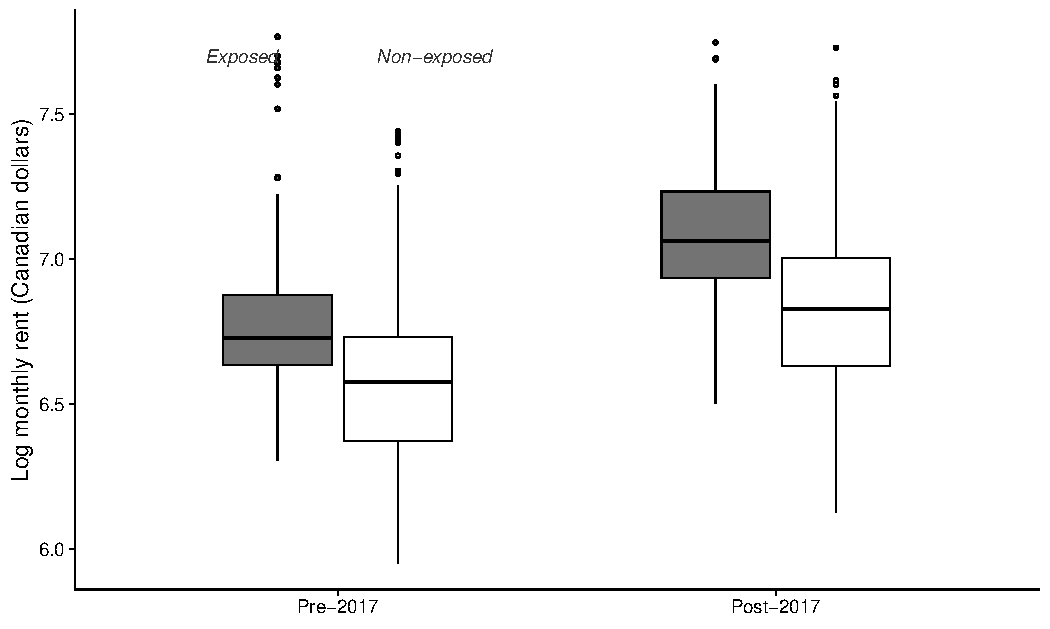
\includegraphics[width=0.78\textwidth]{figures/fig_rent_distribution}
  \par\smallskip\begin{minipage}{0.78\textwidth}\setstretch{1.0}\footnotesize\textit{Notes:} Boxplots of log monthly rent over all city-year observations in the main
    sample, partitioned by exposure status
    ($s_{WL,d}>0$ versus $s_{WL,d}=0$) and by period
    (pre-2017: 2008--2016; post-2017: 2017--2024).
    The dependent variable is log monthly rent for two-bedroom apartments in
    buildings with at least three units.\end{minipage}
\end{center}

\begin{center}
\begin{minipage}{0.78\textwidth}
\centering\singlespacing
\captionof{figure}{Distribution of Pre-Fire Williams Lake Migration Shares}
\label{fig:treatment_intensity}

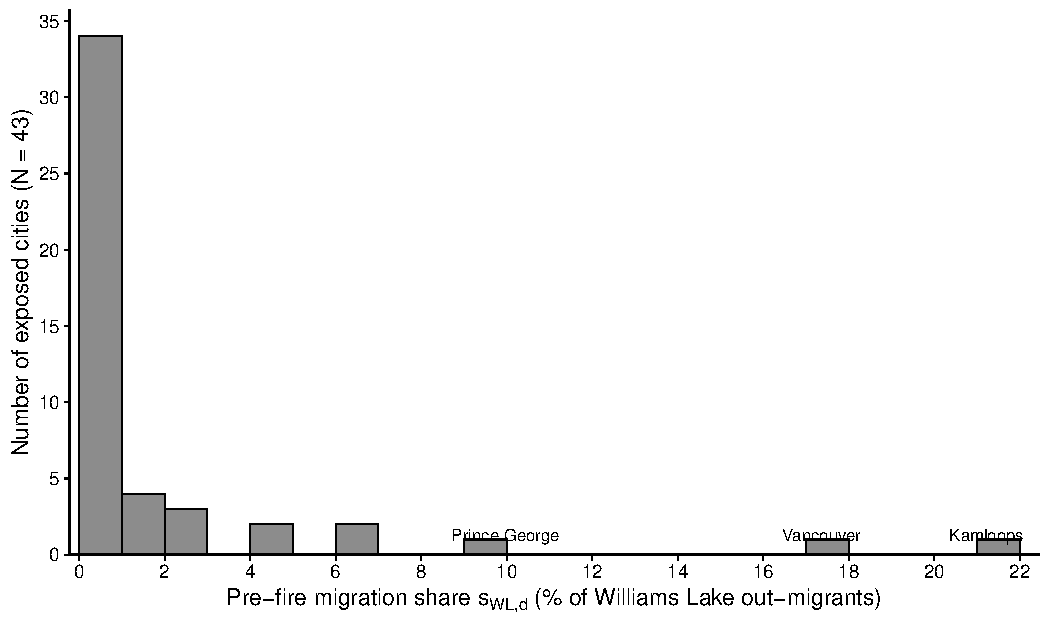
\includegraphics[
  width=\linewidth,
  height=0.38\textheight,
  keepaspectratio
]{figures/fig_treatment_intensity}

\par\smallskip
\setstretch{1.0}
\footnotesize
\textit{Notes:} Histogram of pre-fire migration shares $s_{WL,d}$ across the 43 cities with
strictly positive exposure. The share is defined as the fraction of Williams Lake
out-migrants directed to city $d$ during the 2016/2017 Statistics Canada migration
wave, after excluding rural residual destinations and renormalising shares across
retained city destinations. Cities with $s_{WL,d}=0$ are not displayed.
\end{minipage}
\end{center}
Appendix Figure~\ref{fig:migration_event_studies}repeats the same diagnostic for
the Quesnel placebo origin. They visualise the flow evidence summarised in
Section~\ref{sec:channel} without adding identification beyond
Table~\ref{tab:channel_validation}.

\begin{center}
\begin{minipage}{0.92\textwidth}
\centering\singlespacing
\captionof{figure}{Annual Arrivals Event Studies}
\label{fig:migration_event_studies}

\textbf{Panel A. Williams Lake Origin}\\[0.25em]
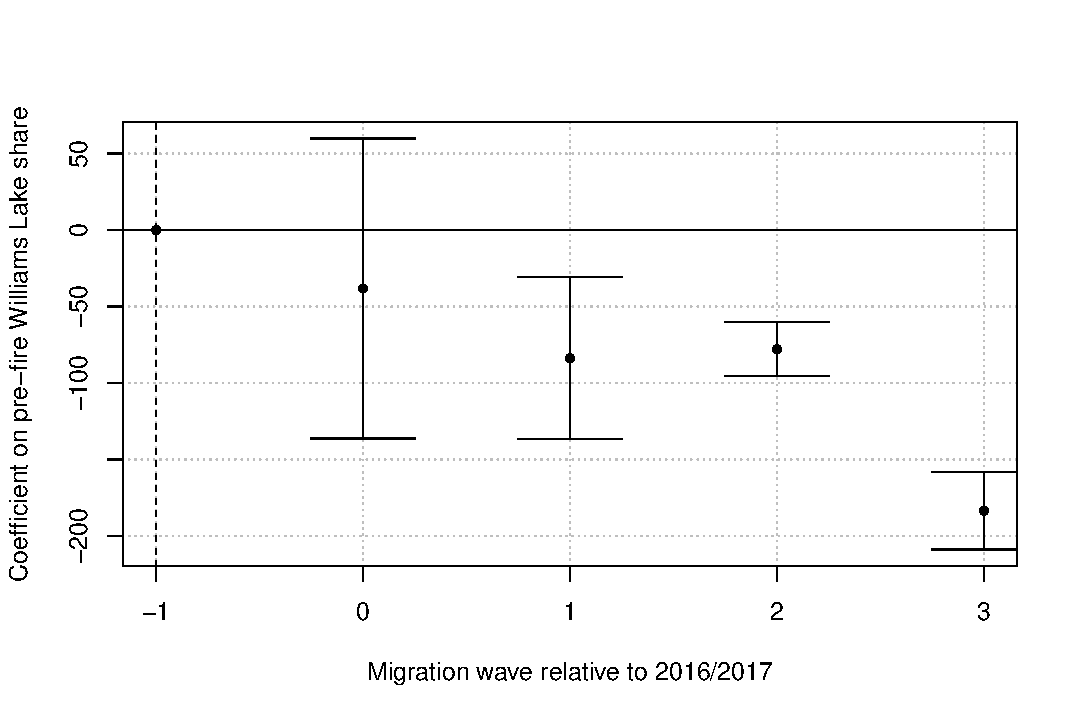
\includegraphics[
  width=0.82\linewidth,
  height=0.27\textheight,
  keepaspectratio
]{figures/event_study_migration_wl}

\vspace{0.5em}

\textbf{Panel B. Quesnel Placebo Origin}\\[0.25em]
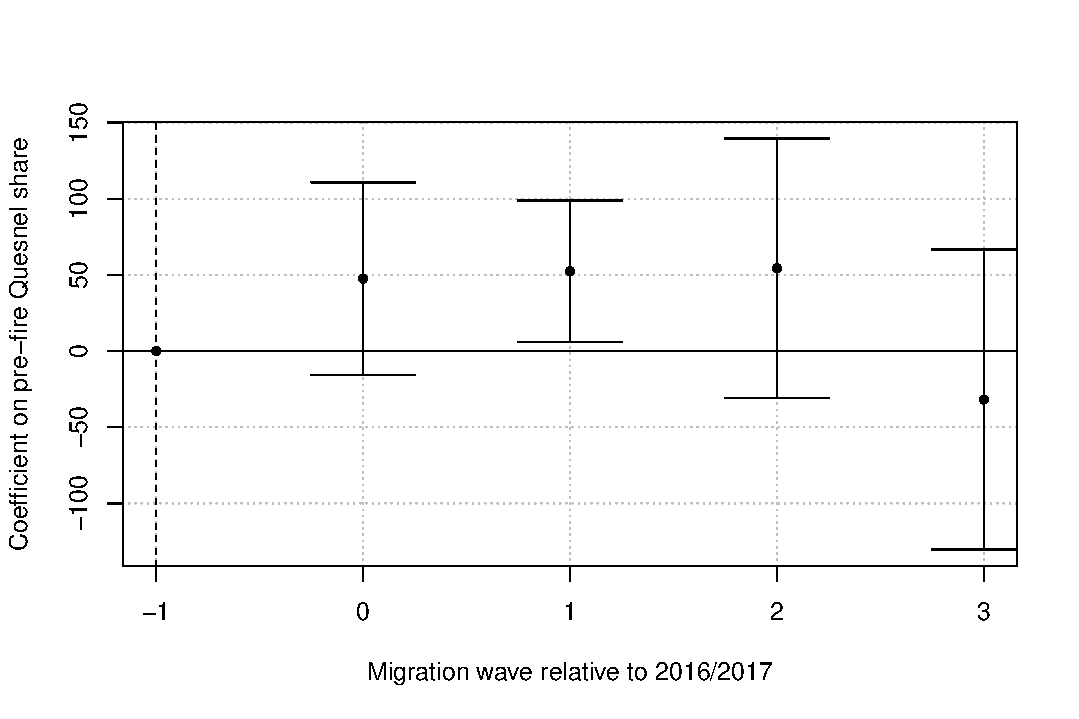
\includegraphics[
  width=0.82\linewidth,
  height=0.27\textheight,
  keepaspectratio
]{figures/event_study_migration_quesnel}

\par\smallskip
\setstretch{1.0}
\footnotesize
\textit{Notes:} Panel A reports coefficients on $s_{WL,d}$ interacted with annual
migration-wave indicators, from an OLS regression of annual bilateral arrivals
from Williams Lake on destination-city and wave fixed effects. Panel B repeats
the same diagnostic for Quesnel, a British Columbia forestry town that did not
experience a wildfire in 2017. The omitted reference wave is 2016/2017.
Shaded bands denote 95\% confidence intervals. Standard errors are clustered
at the destination-city level. Sample: waves 2016/2017--2020/2021.
\end{minipage}
\end{center}

\FloatBarrier

\phantomsection
\subsection*{A.2\quad Identification Diagnostics}
\label{sec:appendix_iv}

Table~\ref{tab:rambachan_roth} reports uniformly valid 95\% confidence sets for
the average post-2017 event-study effect under the honest-inference framework of
\citet{rambachan2023}. The summary statistic averages post-fire coefficients
over $k=1,\ldots,7$ and assigns zero weight to $k=0$, because the 2017 rent
observation is measured only a few months after the July evacuation. The
restriction parameter $\bar{M}$ governs how large post-treatment violations of
parallel trends may be relative to the largest pre-treatment deviation. The case
$\bar{M}=0$ reproduces exact parallel trends. Larger values allow increasingly
severe post-treatment departures from that benchmark. The breakdown value
$\bar{M}^{*}$ is the smallest value at which the confidence set includes zero. In
this application, $\bar{M}^{*}=0.38$, which indicates that the positive
post-2017 event-study pattern is not robust to even moderately larger violations
than those observed before treatment.

\begin{table}[!htbp]
   \centering
   \begin{threeparttable}
   \caption{\label{tab:rambachan_roth} Sensitivity to Parallel-Trend Violations: Rambachan--Roth Confidence Sets}
   \small
   \begin{tabular}{lcc}
      \toprule
      \multicolumn{3}{l}{\textit{Dependent variable: log monthly rent, two-bedroom apartments, buildings $\geq 3$ units.}} \\
      \multicolumn{3}{l}{\textit{Rambachan--Roth (2023) sensitivity analysis.}} \\
      \addlinespace
      Trend violation $\bar{M}$ & Point estimate & 95\% confidence set \\
      \midrule
      $0.0$ & $0.756$ & $[0.35,\ 1.17]$ \\
      $0.5$ & ---     & $[-0.16,\ 1.93]$ \\
      $1.0$ & ---     & $[-0.94,\ 2.80]$ \\
      $1.5$ & ---     & $[-1.83,\ 3.72]$ \\
      \bottomrule
   \end{tabular}
   \begin{tablenotes}[flushleft]
      \footnotesize
      \item \textit{Notes:} Sensitivity analysis from \citet{rambachan2023} applied
      to the fully interacted rent event study with city and year fixed
      effects ($N=2{,}225$). The target parameter is the average
      post-treatment effect over event times $k=1,\ldots,7$; $k=0$
      receives zero weight because the 2017 Canada Mortgage and Housing
      Corporation rent observation is measured in October, several months
      after the July evacuation.
      $\bar{M}=0$ reports the conventional 95\% confidence interval
      under exact parallel trends. For $\bar{M}>0$, the table reports
      uniformly valid 95\% confidence sets allowing post-treatment
      violations up to $\bar{M}$ times the largest pre-treatment
      deviation. The breakdown value is $\bar{M}^{*}=0.38$, the
      smallest value at which the confidence set first includes zero.
      Standard errors clustered at the city level.
   \end{tablenotes}
   \end{threeparttable}
\end{table}

The main analysis remains in reduced form because the rental panel and the
migration-flow panel do not share a comparable time structure. Canada Mortgage and Housing Corporation rents are
observed annually from 2008 to 2024, while bilateral migration flows are
available only for five waves, from 2016/2017 to 2020/2021. This appendix reports
a limited-window fixed-effects 2SLS exercise to clarify why this paper does not convert the
exposure estimates into an IV elasticity.

The exercise instruments observed annual arrivals from Williams Lake with
$s_{WL,d}\times \mathbf{1}[\text{post-flow wave}]$ and then relates log rent to
fitted arrivals. Two temporal alignments are shown. The concurrent alignment maps
the 2017/2018 migration wave to rent year 2017. The lagged alignment maps that
wave to rent year 2018. The lagged version better respects the fact that the
migration wave extends through June, whereas Canada Mortgage and Housing Corporation rent is measured in October.
Neither mapping is exact.

Table~\ref{tab:iv_limited_window} reports the first stage, the reduced form over
the same short window, and the resulting fixed-effects 2SLS coefficient. The first stage is precisely estimated but negative
($\hat{\eta}=-95.8^{***}$, $F=85.9$). This reproduces the pattern documented in
Section~\ref{sec:channel}. High-share destinations record fewer annual arrivals
from Williams Lake after 2017 than in the share-defining 2016/2017 wave. The
short-window reduced form on rent is positive, with coefficients near $0.49$ and
$0.50$ depending on the alignment. Dividing a positive reduced form by a negative
first stage produces a negative fixed-effects 2SLS coefficient of approximately
$-0.005^{***}$.

\begin{table}[!htbp]
   \centering
   \caption{Exploratory Limited-Window Migration First Stage and FE-2SLS}
   \label{tab:iv_limited_window}
   \footnotesize
   \resizebox{\textwidth}{!}{%
   \begin{tabular}{lrrrrrr}
      \toprule
      & \multicolumn{3}{c}{Wave 2017/18 $\to$ Rent 2017}
      & \multicolumn{3}{c}{Wave 2017/18 $\to$ Rent 2018} \\
      \cmidrule(lr){2-4} \cmidrule(lr){5-7}
      & (1) First stage & (2) Reduced form & (3) FE-2SLS
      & (4) First stage & (5) Reduced form & (6) FE-2SLS \\
      \addlinespace
      \textit{Dependent variable:}
      & \textit{Arrivals} & \textit{Log rent} & \textit{Log rent}
      & \textit{Arrivals} & \textit{Log rent} & \textit{Log rent} \\
      \midrule
      $s_{WL,d} \times \mathrm{PostFlow}$
         & $-$95.80$^{***}$ & 0.492$^{***}$ &
         & $-$95.80$^{***}$ & 0.497$^{***}$ & \\
         & (8.940) & (0.134) &
         & (8.940) & (0.137) & \\
      Arrivals from Williams Lake
         & & & $-$0.005$^{***}$
         & & & $-$0.005$^{***}$ \\
         & & & (0.002)
         & & & (0.002) \\
      \addlinespace
      Observations      & 655   & 655   & 655   & 655   & 655   & 655 \\
      $R^{2}$           & 0.97  & 0.98  & 0.98  & 0.97  & 0.97  & 0.97  \\
      Within $R^{2}$    & 0.12  & 0.02  & 0.02  & 0.12  & 0.02  & 0.02  \\
      RMSE              & 2.838 & 0.041 & 0.043 & 2.838 & 0.043 & 0.046 \\
      First-stage $F$   &       &       & 85.9  &       &       & 85.9 \\
      \addlinespace
      Destination FE    & $\checkmark$ & $\checkmark$ & $\checkmark$
                        & $\checkmark$ & $\checkmark$ & $\checkmark$ \\
      Year FE           & $\checkmark$ & $\checkmark$ & $\checkmark$
                        & $\checkmark$ & $\checkmark$ & $\checkmark$ \\
      \bottomrule
   \end{tabular}}
   \par\smallskip
   \begin{minipage}{0.96\textwidth}
   \setstretch{1.0}
   \footnotesize
   \textit{Notes:} Columns~(1) and~(4) report first-stage regressions where
   the dependent variable is annual migration arrivals from Williams Lake.
   Columns~(2) and~(5) report reduced-form regressions on log monthly rent
   for two-bedroom apartments in buildings $\geq 3$ units. Columns~(3)
   and~(6) report fixed-effects 2SLS estimates, instrumenting observed
   Williams Lake arrivals with $s_{WL,d}\times\mathrm{PostFlow}$.
   Columns~(1)--(3) align migration wave 2017/2018 with rent year 2017;
   columns~(4)--(6) align the same wave with rent year 2018.
   All specifications include destination-city and year fixed effects.
   Standard errors clustered at the destination-city level in parentheses.
   These estimates are exploratory and are not used as the preferred
   rent-effect specification. * $p<0.10$, ** $p<0.05$, *** $p<0.01$.
   \end{minipage}
\end{table}

That coefficient has no credible structural interpretation in this setting. It
does not imply that additional Williams Lake arrivals lower rents in receiving
cities. Instead, it shows that the available annual migration-flow measure is not
a suitable endogenous regressor for an IV design built around a short-lived
emergency evacuation. The negative first stage also signals a monotonicity failure. Cities with
stronger pre-fire ties to Williams Lake attracted fewer evacuees post-fire
relative to the share-defining wave, leaving no complier population and no
coherent local average treatment effect to recover. The limited flow window also inherits the regional
confounding concerns that affect the main reduced-form design. For these reasons,
the fixed-effects 2SLS exercise is reported as a diagnostic that limits interpretation, not
as a preferred estimate of the effect of displaced households on rents.

\FloatBarrier

\subsection*{A.3\quad Rental-Market Heterogeneity}
\label{app:heterogeneity}

Figure~\ref{fig:heterogeneity_coefplot} reports the complete heterogeneity
results discussed briefly in Section~\ref{sec:results}. Each point is the
coefficient on $Z_{WL}$ from a separate regression with city and year fixed
effects. Vertical lines show 95\% confidence intervals. Standard errors clustered
at the city level. The dashed reference line marks the baseline estimate of
$0.818$ (2 bedrooms, apartment structures $\geq 3$ units). The row structure
column omits the bachelor-unit cell, which is not estimable after balancing
($N_d=2$); the 1-bedroom estimate in that column ($-4.288$, s.e.\ $1.222$)
is driven by only 14 cities and is not interpretable as an economic estimate.

\begin{center}
\singlespacing
\captionof{figure}{Heterogeneity by Unit Type and Housing Structure}
  \label{fig:heterogeneity_coefplot}
  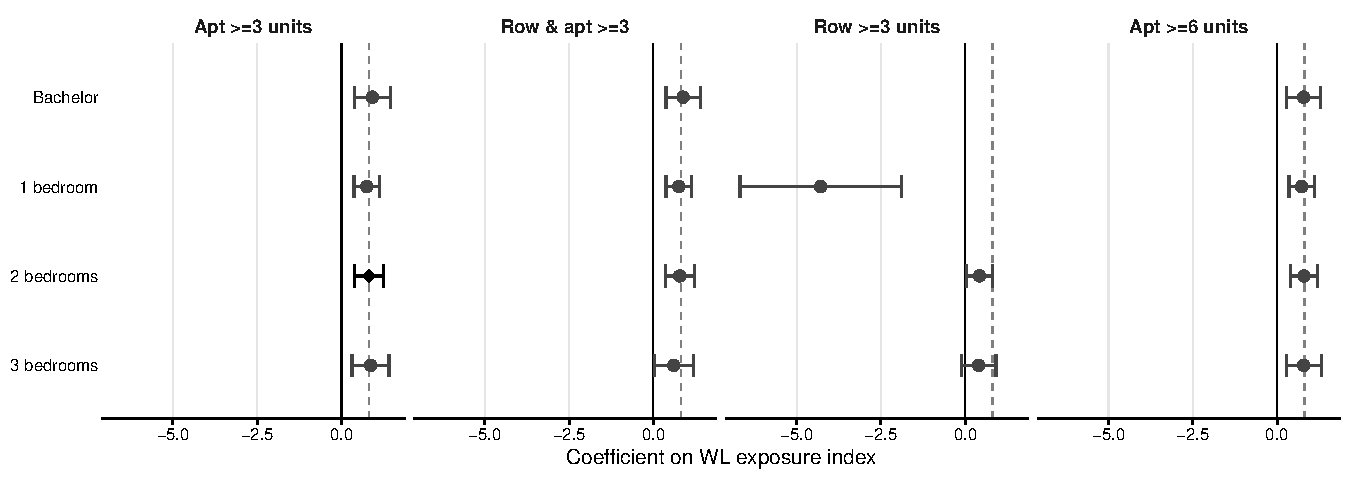
\includegraphics[width=0.95\textwidth]{figures/fig_heterogeneity_coefplot}
  \par\smallskip\begin{minipage}{0.95\textwidth}\setstretch{1.0}\footnotesize\textit{Notes:} Each point is the OLS coefficient on the post-2017 Williams Lake exposure
    index $Z_{WL}$ from a separate regression of log monthly rent on $Z_{WL}$
    with city and year fixed effects. Bars show 95\% confidence intervals.
    Standard errors clustered at the city level. The dashed vertical line marks
    the baseline estimate ($0.818$, 2~bedrooms, apt $\geq 3$ units, diamond).
    Period: 2008--2024.\end{minipage}
\end{center}


\begin{table}[!htbp]
   \centering
   \caption{Exploratory Limited-Window Migration First Stage and FE-2SLS}
   \label{tab:iv_limited_window}
   \footnotesize
   \resizebox{\textwidth}{!}{%
   \begin{tabular}{lrrrrrr}
      \toprule
      & \multicolumn{3}{c}{Wave 2017/18 $\to$ Rent 2017}
      & \multicolumn{3}{c}{Wave 2017/18 $\to$ Rent 2018} \\
      \cmidrule(lr){2-4} \cmidrule(lr){5-7}
      & (1) First stage & (2) Reduced form & (3) FE-2SLS
      & (4) First stage & (5) Reduced form & (6) FE-2SLS \\
      \addlinespace
      \textit{Dependent variable:}
      & \textit{Arrivals} & \textit{Log rent} & \textit{Log rent}
      & \textit{Arrivals} & \textit{Log rent} & \textit{Log rent} \\
      \midrule
      $s_{WL,d} \times \mathrm{PostFlow}$
         & $-$95.80$^{***}$ & 0.492$^{***}$ &
         & $-$95.80$^{***}$ & 0.497$^{***}$ & \\
         & (8.940) & (0.134) &
         & (8.940) & (0.137) & \\
      Arrivals from Williams Lake
         & & & $-$0.005$^{***}$
         & & & $-$0.005$^{***}$ \\
         & & & (0.002)
         & & & (0.002) \\
      \addlinespace
      Observations      & 655   & 655   & 655   & 655   & 655   & 655 \\
      $R^{2}$           & 0.97  & 0.98  & 0.98  & 0.97  & 0.97  & 0.97  \\
      Within $R^{2}$    & 0.12  & 0.02  & 0.02  & 0.12  & 0.02  & 0.02  \\
      RMSE              & 2.838 & 0.041 & 0.043 & 2.838 & 0.043 & 0.046 \\
      First-stage $F$   &       &       & 85.9  &       &       & 85.9 \\
      \addlinespace
      Destination FE    & $\checkmark$ & $\checkmark$ & $\checkmark$
                        & $\checkmark$ & $\checkmark$ & $\checkmark$ \\
      Year FE           & $\checkmark$ & $\checkmark$ & $\checkmark$
                        & $\checkmark$ & $\checkmark$ & $\checkmark$ \\
      \bottomrule
   \end{tabular}}
   \par\smallskip
   \begin{minipage}{0.96\textwidth}
   \footnotesize
   \textit{Notes:} Columns~(1) and~(4): first-stage regressions where the
   dependent variable is annual migration arrivals from Williams Lake.
   Columns~(2) and~(5): reduced-form regressions on log monthly rent
   for two-bedroom apartments in buildings $\geq 3$ units. Columns~(3)
   and~(6): FE-2SLS second stage; observed Williams Lake arrivals
   instrumented by $s_{WL,d} \times \mathrm{PostFlow}$. Columns~(1)--(3)
   align migration wave 2017/2018 with rent year 2017; columns~(4)--(6)
   align the same wave with rent year 2018. All specifications include
   destination-city and year fixed effects. Standard errors clustered at the
   destination-city level in parentheses. These estimates are exploratory.
   * $p < 0.10$, ** $p < 0.05$, *** $p < 0.01$.
   \end{minipage}
\end{table}

The supply-elasticity estimates in \citet{saiz2010} imply that rent responses to housing-demand shocks are two to
three times larger in cities where supply is physically or regulatorily
constrained. This prediction is directly testable in the shift-share design by
interacting the exposure index with a proxy for supply inelasticity. Because the
Canadian equivalent of the Wharton Residential Land Use Regulatory Index is not
available for all 131 cities, I use the average pre-fire rent level (2008--2016)
as a proxy. Cities with historically higher rents face more supply-constrained
conditions, consistent with a Saiz-type mechanism.

Let $\mathrm{Tight}_d = \mathbf{1}[\bar{R}_{d,\text{pre}} \geq \$775]$, where
\$775 is the sample median pre-fire rent. The extended specification is:
\begin{equation}
\log R_{dt} = \alpha + \pi_1 Z_{WL,dt} + \pi_2\,(Z_{WL,dt}\times\mathrm{Tight}_d)
              + \gamma_d + \lambda_t + \varepsilon_{dt}.
\label{eq:supply_het}
\end{equation}
Equation~\eqref{eq:supply_het} nests the baseline specification~\eqref{eq:main} when $\pi_2=0$. The Saiz prediction is $\hat{\pi}_2 > 0$.

Table~\ref{tab:supply_het} reports the results. The interaction term is
$\hat{\pi}_2 = 0.007$ (s.e.\ $0.547$), statistically indistinguishable from
zero. The point estimates across tight and slack subsamples are nearly
identical ($0.836$ vs.\ $0.784$); the difference in statistical significance
between the two subsamples reflects sample size and precision, not heterogeneous
treatment effects. The Saiz~(2010) supply-elasticity prediction is therefore
not validated by this design.

\begin{table}[!htbp]
  \centering
  \caption{Supply-Side Heterogeneity: Tight vs.\ Slack Markets}
  \label{tab:supply_het}
  \footnotesize

  \resizebox{\textwidth}{!}{%
  \begin{tabular}{lccc}
    \toprule
    & (1) & (2) & (3) \\
    & Interaction & Tight markets & Slack markets \\
    \midrule
    $Z_{WL}$ 
      & 0.812 & 0.836$^{***}$ & 0.784 \\
      & (0.504) & (0.265) & (0.484) \\
    $Z_{WL} \times \mathrm{Tight}_d$
      & 0.007 & & \\
      & (0.547) & & \\
    \addlinespace
    Observations
      & 2{,}225 & 1{,}122 & 1{,}103 \\
    $R^{2}$
      & 0.940 & 0.865 & 0.944 \\
    Within $R^{2}$
      & 0.021 & 0.026 & 0.010 \\
    \addlinespace
    City FE
      & $\checkmark$ & $\checkmark$ & $\checkmark$ \\
    Year FE
      & $\checkmark$ & $\checkmark$ & $\checkmark$ \\
    \bottomrule
  \end{tabular}
  }

  \par\smallskip
  \begin{minipage}{0.96\textwidth}
  \setstretch{1.0}
  \footnotesize
  \textit{Notes:} This table reports reduced-form exposure estimates. The dependent
  variable is log monthly rent for two-bedroom apartments in buildings with at
  least three units. Tight markets are cities with mean 2008--2016 rent above
  the sample median (\$775). Column~(1) estimates the pooled interaction
  specification with $Z_{WL,dt}\times\mathrm{Tight}_d$, where
  $\mathrm{Tight}_d=\mathbf{1}[\bar{R}_{d,\mathrm{pre}}\geq\$775]$.
  Columns~(2)--(3) estimate the baseline specification separately for tight
  and slack markets. All specifications include city and year fixed effects.
  Standard errors are clustered at the city level in parentheses.
  * $p<0.10$, ** $p<0.05$, *** $p<0.01$.
  \end{minipage}
\end{table}

This null is itself informative. Two interpretations are consistent with it.
First, the residual identifying variation, once city and year fixed effects
are absorbed, may be insufficient to detect effect heterogeneity of
plausible magnitude across the two subsamples. Second, if the baseline estimate
reflects provincial confounding rather than a genuine displacement channel,
there is no theoretical reason to expect it to be larger in supply-constrained
markets; regional rent trends need not respect supply-elasticity gradients.
The null interaction result is therefore consistent with the regional
confounding hypothesis as well as with a genuine but homogeneous displacement
effect.

Figure~\ref{fig:heterogeneity_all_dims} plots the exposure coefficient across
three remaining heterogeneity dimensions, covering city size (small, medium,
large), geographic region (West, East), and housing supply tightness following
\citet{saiz2010}. The figure reports all subgroup cuts regardless of statistical
significance.

\begin{center}
\begin{minipage}{0.86\textwidth}
\centering\singlespacing
\captionof{figure}{Heterogeneity by City Size, Region, and Housing Supply Constraints}
\label{fig:heterogeneity_all_dims}

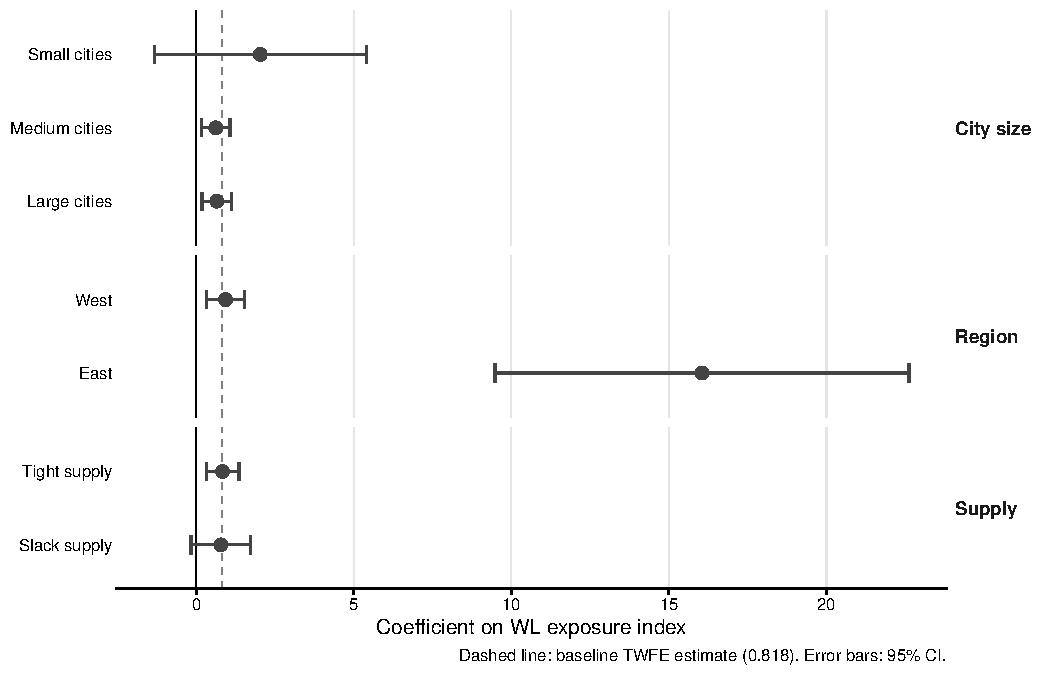
\includegraphics[
  width=\linewidth,
  height=0.34\textheight,
  keepaspectratio
]{figures/fig_heterogeneity_all_dims}

\par\smallskip
\setstretch{1.0}
\footnotesize
\textit{Notes:} Each point reports the reduced-form coefficient on the
post-2017 Williams Lake exposure index across seven subgroups. Bars show
95\% confidence intervals. Standard errors are clustered at the city level.
The dashed vertical line marks the baseline reduced-form estimate ($0.818$,
full sample, column~4 of Table~\ref{tab:main_result}). City size is defined
as small ($<$50{,}000), medium (50{,}000--200{,}000), and large
($>$200{,}000). Region is West (BC, AB, SK, MB) or East. Supply tightness
is defined by pre-2017 average rent above or below the sample median,
following \citet{saiz2010}. Benjamini-Hochberg adjusted p-values are
reported in the figure source file; five of seven subgroup estimates survive
correction at $q<0.05$. Period: 2008--2024.
\end{minipage}
\end{center}
\FloatBarrier

\subsection*{A.4\quad Exposure, Influence, and Robustness}
\label{app:exposure_influence}

Table~\ref{tab:rotemberg} reports Rotemberg weights for each exposed city.
In this single-shock shift-share design, the weight of city~$d$ is proportional to
$s_{WL,d}^2$ \citep{goldsmith2020}. Kamloops and Vancouver together account for
roughly 40~percent of total identification weight; the top five cities account for
approximately 60~percent.

\begin{table}[!htbp]
  \caption{Rotemberg Weights by Pre-Fire Exposure Rank}
  \label{tab:rotemberg}
  \centering\small
  \begin{threeparttable}
  \begin{tabular}{lrrrr}
    \toprule
    City & $s_{WL,d}$ (\%) & $s_{WL,d}^2$ & $w_d^R$ (\%) & Cumulative (\%) \\
    \midrule
    Kamloops & 21.22 & 0.0450 & 43.97 & 43.97 \\
    Vancouver & 17.36 & 0.0301 & 29.43 & 73.40 \\
    Prince George & 9.97 & 0.0099 & 9.70 & 83.10 \\
    Kelowna & 6.91 & 0.0048 & 4.67 & 87.77 \\
    Quesnel & 6.75 & 0.0046 & 4.45 & 92.22 \\
    Abbotsford--Mission & 4.98 & 0.0025 & 2.43 & 94.65 \\
    Vernon & 4.18 & 0.0017 & 1.71 & 96.35 \\
    Calgary & 2.57 & 0.0007 & 0.65 & 97.00 \\
    Victoria & 2.57 & 0.0007 & 0.65 & 97.64 \\
    Campbell River & 2.41 & 0.0006 & 0.57 & 98.21 \\
    \addlinespace
    \textit{All other cities ($N=38$)} & 21.06 & --- & 1.79 & 100.00 \\
    \bottomrule
  \end{tabular}
  \begin{tablenotes}[flushleft]\footnotesize
    \item \textit{Notes:} Rotemberg weights $w_d^R = s_{WL,d}^2 / \sum_{d'} s_{WL,d'}^2$
      \citep{goldsmith2020}. In this balanced panel with a single binary Post indicator,
      these weights equal the squared pre-fire migration share normalised to sum to one
      across the 43 exposed cities. Each weight measures city~$d$'s contribution to the
      overall identification of $\hat{\pi}$. Non-exposed cities ($s_{WL,d}=0$) carry zero
      Rotemberg weight and serve as the comparison group, not as identifying variation.
  \end{tablenotes}
  \end{threeparttable}
\end{table}

The economic implication of this concentration is stark. The coefficient
$\hat\pi$ is effectively a weighted average of post-2017 rent differentials
across exposed cities, with Kamloops and Vancouver together accounting for
nearly half the signal. Kamloops is a mid-sized Interior city that also
experienced strong population growth and housing demand from in-migration
unrelated to the wildfire. Vancouver is Canada's most supply-constrained
rental market and was simultaneously affected by the Foreign Buyers Tax
(August 2016) and subsequent demand displacement toward rentals. If either
city's post-2017 rent trajectory reflects forces specific to that city rather
than the wildfire exposure channel, the aggregate coefficient will be
contaminated. The leave-one-out diagnostics in Figure~\ref{fig:loo_coefplot}
show that removing Kamloops raises rather than lowers the estimate, which
argues against a single-city story but does not resolve the broader
identification question. The honest interpretation is that $\hat\pi$ is
largely identified by what happened in two or three cities with particular
economic histories during a period of broader provincial rental-market
pressure.

Figure~\ref{fig:loo_coefplot} reports the leave-top-$k$ influence diagnostics.
The coefficient rises monotonically from the baseline ($0.818$) as the most
exposed cities are dropped. Removing Kamloops alone raises it to $1.100$, and
dropping the ten most exposed cities yields $5.420$ (s.e.\ $2.700$). This
pattern reflects a non-monotone relationship between exposure and the
post-2017 rent outcome. Once Kamloops is excluded, medium-exposure cities
in the range $s_{WL,d}\in[0.03,0.10]$ dominate and exhibit a stronger
per-unit relationship. As the top-$k$ cities are progressively removed, the
exposure variance in the denominator shrinks mechanically, inflating the
normalised coefficient. The result argues against a single-city story but does
not resolve the regional confounding concern.

\subsubsection*{A.4a\quad TWFE Weights and the Negative-Weight Concern}
\label{app:twfe_weights}

\citet{dechaisemartin2020} show that the two-way fixed effects estimator can
assign negative weights to some average treatment effects when those effects are
heterogeneous across treatment intensities. For the continuous exposure index
$Z_{WL,dt}=s_{WL,d}\times\mathbf{1}[t\geq 2017]$, this concern is addressed
analytically. By the Frisch-Waugh-Lovell theorem, the TWFE estimator projects
$\log R_{dt}$ onto the within-transformed regressor
$\tilde{Z}_{WL,dt}=Z_{WL,dt}-\bar{Z}_{WL,d}-\bar{Z}_{WL,t}+\bar{Z}_{WL}$.
Substituting $Z_{WL,dt}=s_{WL,d}\times\mathrm{Post}_{t}$ yields
\[
\tilde{Z}_{WL,dt}
  = (s_{WL,d}-\bar{s})\times\Bigl(\mathrm{Post}_{t}-\tfrac{T^{\mathrm{post}}}{T}\Bigr),
\]
where $\bar{s}$ is the cross-city mean of the exposure share and
$T^{\mathrm{post}}/T=8/17$ for the 2008--2024 panel. The TWFE weight of cell
$(d,t)$ is $w_{dt}\propto\tilde{Z}_{WL,dt}^{2}\geq 0$ for all $(d,t)$.
The simultaneous shock and the time-invariant post-treatment intensity guarantee
non-negative weights by construction, so $\hat{\pi}$ is a non-negatively
weighted average of city-level rent differentials. Figure~\ref{fig:twfe_weights}
displays the implied weight distribution across exposed cities, which closely
mirrors the Rotemberg weights reported in Table~\ref{tab:rotemberg}: Kamloops and
Vancouver together account for approximately 77~percent of the identifying
variation. The replication script (\texttt{twfe\_diag.R}) verifies this result
numerically.

\begin{center}
\singlespacing
\captionof{figure}{TWFE Identification Weights by Exposed City}
\label{fig:twfe_weights}
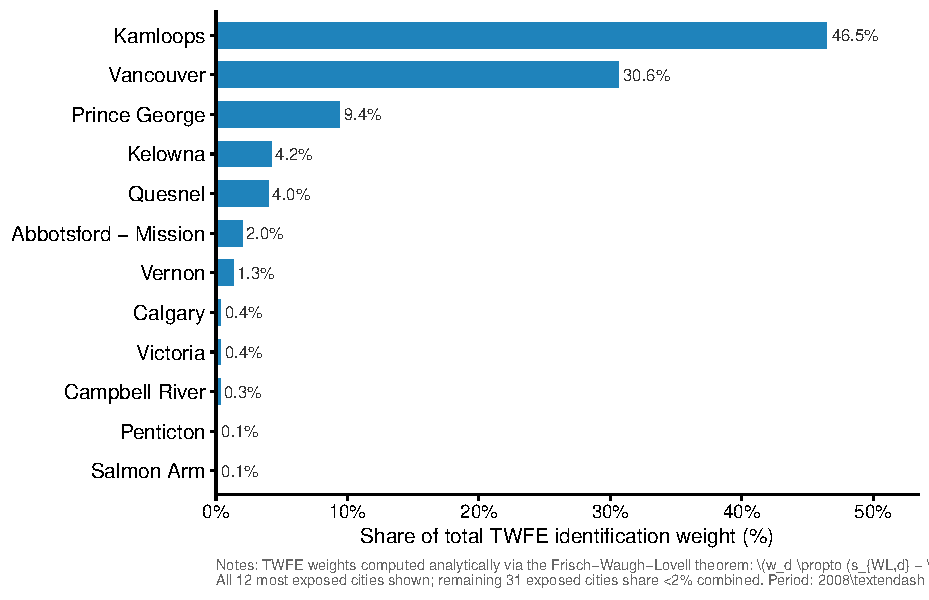
\includegraphics[width=0.74\textwidth]{figures/fig_twfe_weights}
\par\smallskip
\begin{minipage}{0.74\textwidth}\setstretch{1.0}\footnotesize
\textit{Notes:} Frisch-Waugh-Lovell identification weights
$w_d\propto(s_{WL,d}-\bar{s})^{2}$, normalised to sum to 100~percent
across the 43 exposed cities ($s_{WL,d}>0$).
Non-exposed cities carry zero weight and serve as the comparison group.
$\bar{s}=0.0074$ (cross-city mean of the pre-fire exposure share).
Period: 2008--2024.
\end{minipage}
\end{center}

\begin{center}
\singlespacing
\captionof{figure}{Leave-One-Out Influence Diagnostics}
  \label{fig:loo_coefplot}
  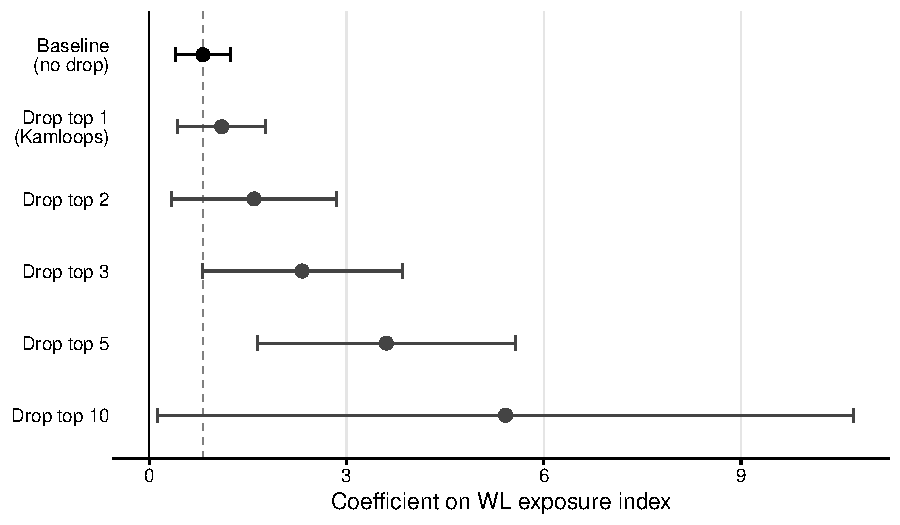
\includegraphics[width=0.78\textwidth]{figures/fig_loo_coefplot}
  \par\smallskip\begin{minipage}{0.78\textwidth}\setstretch{1.0}\footnotesize\textit{Notes:} Each point is the OLS coefficient on $Z_{WL}$ after sequentially dropping
    the top $k$ cities by pre-fire exposure rank, with 95\% confidence intervals.
    The dashed vertical line marks the baseline estimate ($0.818$, full sample).
    Standard errors clustered at the city level. Dependent variable: log monthly
    rent, two-bedroom apartments, buildings $\geq 3$ units. Period: 2008--2024.\end{minipage}
\end{center}

Table~\ref{tab:robustness_instrument} collects secondary exposure and
sample checks, including the Fort McMurray-only estimate, the joint WL+FM
specification, the aggregated exposure index, and the unbalanced-panel
re-estimation.

\begin{table}[!htbp]
   \caption{\label{tab:robustness_instrument} Robustness: Alternative Exposure Specifications}
   \centering\small
   \resizebox{\textwidth}{!}{%
   \begin{threeparttable}
   \begin{tabular}{lrrrrr}
      \toprule
      \multicolumn{6}{l}{\textit{Dependent variable: log monthly rent, two-bedroom apartments, buildings $\geq 3$ units. Reduced-form exposure specification estimated by OLS..}} \\
      \addlinespace
                         & (1) Baseline & (2) FM only & (3) WL+FM & (4) Aggregated & (5) Unbalanced \\
      \midrule
      $Z_{WL}$ (BC 2017) & 0.818$^{***}$ &             & 0.835$^{***}$ &               & 0.828$^{***}$ \\
                         & (0.216)       &             & (0.234)       &               & (0.218) \\
      \addlinespace
      $Z_{FM}$ (Fort McMurray 2016)
                         &               & 0.055       & $-$0.670      &               & \\
                         &               & (1.000)     & (0.813)       &               & \\
      \addlinespace
      $\hat{Z}$ (aggregated)
                         &               &             &               & 0.637$^{***}$ & \\
                         &               &             &               & (0.169)       & \\
      \addlinespace
      Observations       & 2,225         & 2,242       & 2,242         & 2,242         & 2,382 \\
      $R^{2}$            & 0.94          & 0.95        & 0.95          & 0.95          & 0.94  \\
      Within $R^{2}$     & 0.02          & $<$0.001    & 0.03          & 0.02          & 0.02  \\
      RMSE               & 0.075         & 0.069       & 0.068         & 0.069         & 0.075 \\
      \addlinespace
      City FE            & $\checkmark$  & $\checkmark$ & $\checkmark$ & $\checkmark$  & $\checkmark$ \\
      Year FE            & $\checkmark$  & $\checkmark$ & $\checkmark$ & $\checkmark$  & $\checkmark$ \\
      \bottomrule
   \end{tabular}
   \begin{tablenotes}[flushleft]
      \footnotesize
      \item \textit{Notes:} Dependent variable: log monthly rent, two-bedroom apartments,
      buildings $\geq 3$ units. OLS: ordinary least squares. FE: fixed effects. FM: Fort McMurray. WL: Williams Lake.
      $Z_{WL} = s_{WL,d} \times \mathrm{Post}_{2017}$: Williams Lake
      shift-share exposure index (observed pre-fire shares).
      $Z_{FM}$: Fort McMurray exposure index (gravity-predicted shares
      $\times$ $\mathrm{Post}_{2016}$).
      $\hat{Z} = Z_{WL} + Z_{FM}$: aggregated exposure.
      Column~(1): main panel of 131 cities ($N=2{,}225$).
      Columns~(2)--(4): panel augmented with Fort McMurray destinations
      ($N=2{,}242$). Column~(5): unbalanced panel ($N=2{,}382$).
      All specifications include city and year fixed effects.
      Standard errors clustered at the city level in parentheses.
      Period: 2008--2024.

      * $p < 0.10$, ** $p < 0.05$, *** $p < 0.01$.
   \end{tablenotes}
   \end{threeparttable}}
\end{table}

Table~\ref{tab:robustness_clustering} verifies that the baseline inference is not sensitive to the choice of clustering level. The baseline clusters at the city level (131 clusters). Province-level clustering (10 clusters) and two-way clustering at the city-by-year level are both more demanding and produce slightly wider standard errors, but the coefficient on $Z_{WL}$ remains statistically significant at the one-percent level across all specifications. Population-weighted and rent-weighted OLS yield point estimates close to the baseline. The evidence in this table supports reading the main result as an inference that is stable across plausible clustering assumptions.

\begin{table}[!htbp]
  \caption{Robustness: Alternative Standard Errors and Weighting}
  \label{tab:robustness_clustering}
  \centering\small
  \resizebox{\textwidth}{!}{%
  \begin{threeparttable}
    \begin{tabular}{lrrrrr}
      \toprule
      \multicolumn{6}{l}{\textit{Dependent variable: log monthly rent, two-bedroom apartments,
        buildings $\geq 3$ units. Reduced-form exposure specification estimated by OLS..}} \\
      \addlinespace
                         & (1)           & (2)           & (3)           & (4)           & (5) \\
                         & Baseline      & Cluster:      & Cluster:      & WLS           & WLS \\
                         & city cluster  & province      & city $\times$ year & population & rent 2008 \\
      \midrule
      $Z_{WL}$ (BC 2017) & 0.818$^{***}$ & 0.818$^{***}$ & 0.818$^{***}$ & 0.543$^{***}$ & 0.892$^{***}$ \\
                         & (0.216)       & (0.157)       & (0.235)       & (0.084)       & (0.248) \\
      \addlinespace
      Observations       & 2{,}225       & 2{,}225       & 2{,}225       & 2{,}225       & 2{,}225 \\
      $R^{2}$            & 0.940         & 0.940         & 0.940         & 0.977         & 0.917 \\
      Within $R^{2}$     & 0.021         & 0.021         & 0.021         & 0.075         & 0.021 \\
      \addlinespace
      City FE            & $\checkmark$  & $\checkmark$  & $\checkmark$  & $\checkmark$  & $\checkmark$ \\
      Year FE            & $\checkmark$  & $\checkmark$  & $\checkmark$  & $\checkmark$  & $\checkmark$ \\
      \bottomrule
    \end{tabular}
    \begin{tablenotes}[flushleft]\footnotesize\setstretch{1.0}
      \item \textit{Notes:} Dependent variable: log monthly rent, two-bedroom apartments,
        buildings $\geq 3$ units.
        Column~(1): baseline specification with standard errors clustered at the city level (131 clusters).
        Column~(2): standard errors clustered at the province level (10 clusters).
        Column~(3): two-way clustering at city and year levels.
        Columns~(4)--(5): weighted least squares; column~(4) weights by city population,
        column~(5) by 2008 rent level.
        Point estimates are identical across columns~(1)--(3) because the coefficient is
        the same regardless of the variance estimator; the spread in standard errors reflects
        clustering assumptions only.
        All specifications include city and year fixed effects.
        * $p < 0.10$, ** $p < 0.05$, *** $p < 0.01$.
    \end{tablenotes}
  \end{threeparttable}}
\end{table}

\FloatBarrier

\subsection*{A.5\quad Fort McMurray Contrast}
\label{app:fort_mcmurray}

The Fort McMurray exercise remains a secondary comparison. It documents a contrast
between Williams Lake exposure and a gravity-predicted Fort McMurray exposure
profile, but it does not identify a duration mechanism. The gravity-predicted
Fort McMurray exposure profile is used as a descriptive comparison; it is not
interpreted as establishing a causal first stage.


Appendix Figure~\ref{fig:gravity_validation} compares observed and gravity-predicted
migration shares for Williams Lake and Fort McMurray. The comparison is diagnostic:
it shows whether the exposure profiles are consistent with standard gravity forces
rather than idiosyncratic destination choices.

\begin{center}
\singlespacing
\captionof{figure}{Gravity Model Validation for Wildfire-Origin Migration Shares}
\label{fig:gravity_validation}
\label{fig:validation_wl}
\label{fig:validation_fm}

\begin{minipage}[t]{0.48\textwidth}
  \centering
  \textbf{Panel A. Williams Lake}\\[0.35em]
  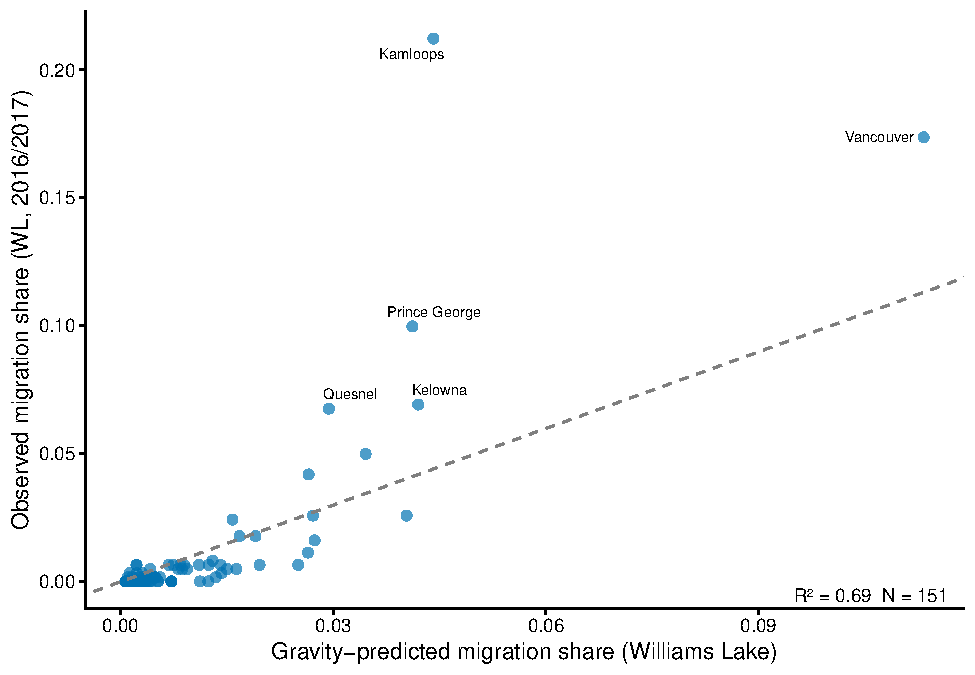
\includegraphics[width=\linewidth]{figures/validation_williams_lake}
\end{minipage}
\hfill
\begin{minipage}[t]{0.48\textwidth}
  \centering
  \textbf{Panel B. Fort McMurray}\\[0.35em]
  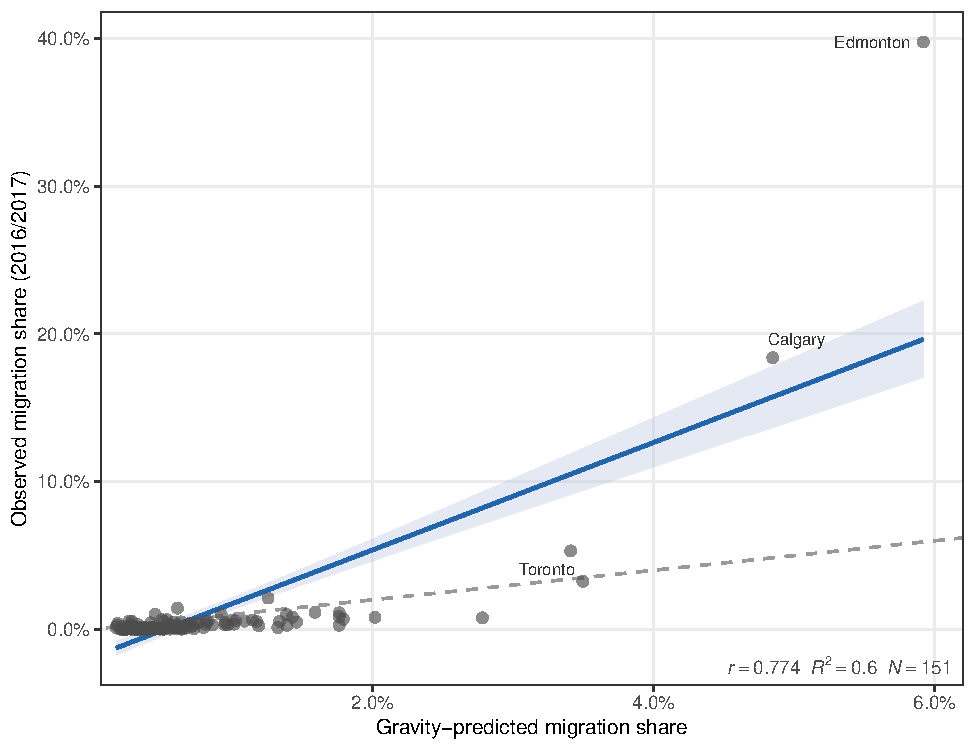
\includegraphics[width=\linewidth]{figures/validation_fort_mcmurray}
\end{minipage}

\par\smallskip
\begin{minipage}{0.96\textwidth}
\setstretch{1.0}
\footnotesize
\textit{Notes:} Panel A plots observed pre-fire Williams Lake migration shares
against gravity-predicted shares constructed from destination population and
bilateral distance. Panel B repeats the same exercise for Wood Buffalo
(Fort McMurray). Each point is a city in the analytical sample. Gravity
predictions are used as exposure diagnostics and are not interpreted as causal
first stages.
\end{minipage}
\end{center}

\begin{center}
\begin{minipage}{0.82\textwidth}
\centering\singlespacing
\captionof{figure}{Event Study: Fort McMurray 2016}
\label{fig:event_study_fm}

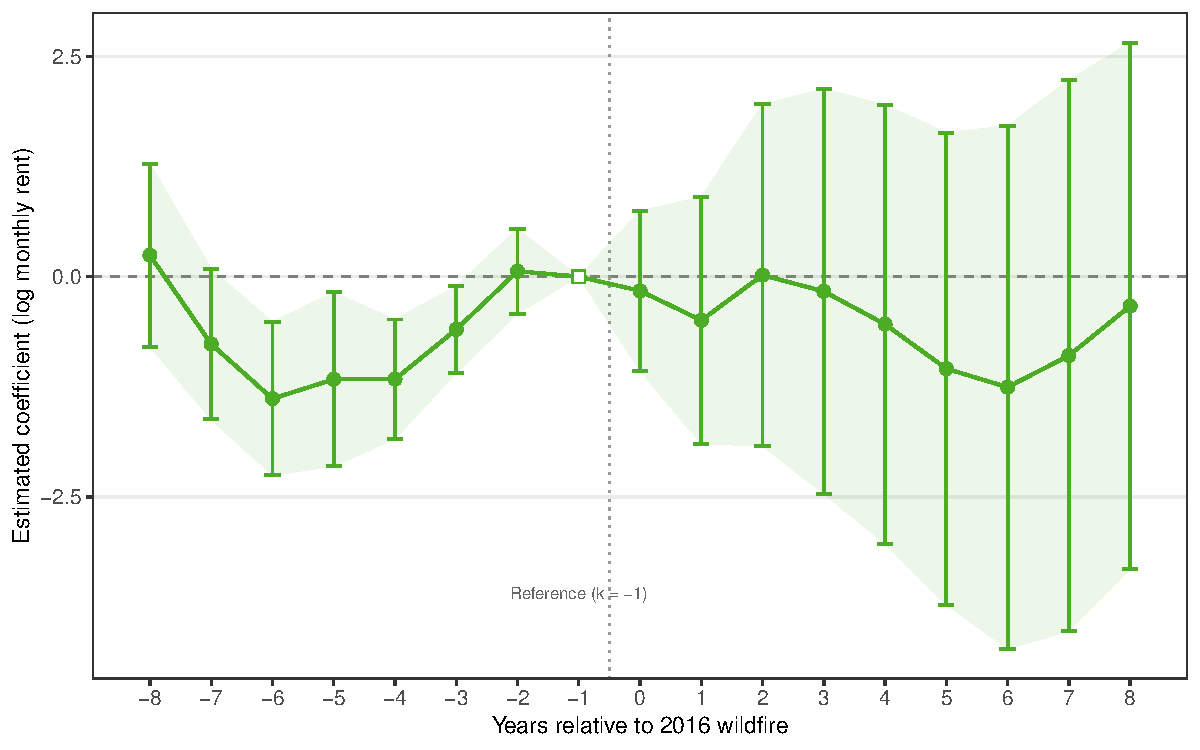
\includegraphics[
  width=\linewidth,
  height=0.36\textheight,
  keepaspectratio
]{figures/event_study_fm_pretrends}

\par\smallskip
\setstretch{1.0}
\footnotesize
\textit{Notes:} Coefficients from a fully interacted specification regressing log
monthly rent on gravity-predicted Fort McMurray exposure interacted
with year indicators, with city and year fixed effects. The omitted
reference year is 2015. Shaded bands denote 95\% confidence intervals.
Standard errors clustered at the city level. Dependent variable: log monthly
rent for two-bedroom apartments in buildings with at least three units.
Period: 2008--2024.
\end{minipage}
\end{center}

\end{document}